\documentclass[twoside]{book}

% Packages required by doxygen
\usepackage{fixltx2e}
\usepackage{calc}
\usepackage{doxygen}
\usepackage[export]{adjustbox} % also loads graphicx
\usepackage{graphicx}
\usepackage[utf8]{inputenc}
\usepackage{makeidx}
\usepackage{multicol}
\usepackage{multirow}
\PassOptionsToPackage{warn}{textcomp}
\usepackage{textcomp}
\usepackage[nointegrals]{wasysym}
\usepackage[table]{xcolor}

% Font selection
\usepackage[T1]{fontenc}
\usepackage[scaled=.90]{helvet}
\usepackage{courier}
\usepackage{amssymb}
\usepackage{sectsty}
\renewcommand{\familydefault}{\sfdefault}
\allsectionsfont{%
  \fontseries{bc}\selectfont%
  \color{darkgray}%
}
\renewcommand{\DoxyLabelFont}{%
  \fontseries{bc}\selectfont%
  \color{darkgray}%
}
\newcommand{\+}{\discretionary{\mbox{\scriptsize$\hookleftarrow$}}{}{}}

% Page & text layout
\usepackage{geometry}
\geometry{%
  a4paper,%
  top=2.5cm,%
  bottom=2.5cm,%
  left=2.5cm,%
  right=2.5cm%
}
\tolerance=750
\hfuzz=15pt
\hbadness=750
\setlength{\emergencystretch}{15pt}
\setlength{\parindent}{0cm}
\setlength{\parskip}{3ex plus 2ex minus 2ex}
\makeatletter
\renewcommand{\paragraph}{%
  \@startsection{paragraph}{4}{0ex}{-1.0ex}{1.0ex}{%
    \normalfont\normalsize\bfseries\SS@parafont%
  }%
}
\renewcommand{\subparagraph}{%
  \@startsection{subparagraph}{5}{0ex}{-1.0ex}{1.0ex}{%
    \normalfont\normalsize\bfseries\SS@subparafont%
  }%
}
\makeatother

% Headers & footers
\usepackage{fancyhdr}
\pagestyle{fancyplain}
\fancyhead[LE]{\fancyplain{}{\bfseries\thepage}}
\fancyhead[CE]{\fancyplain{}{}}
\fancyhead[RE]{\fancyplain{}{\bfseries\leftmark}}
\fancyhead[LO]{\fancyplain{}{\bfseries\rightmark}}
\fancyhead[CO]{\fancyplain{}{}}
\fancyhead[RO]{\fancyplain{}{\bfseries\thepage}}
\fancyfoot[LE]{\fancyplain{}{}}
\fancyfoot[CE]{\fancyplain{}{}}
\fancyfoot[RE]{\fancyplain{}{\bfseries\scriptsize Generated by Doxygen }}
\fancyfoot[LO]{\fancyplain{}{\bfseries\scriptsize Generated by Doxygen }}
\fancyfoot[CO]{\fancyplain{}{}}
\fancyfoot[RO]{\fancyplain{}{}}
\renewcommand{\footrulewidth}{0.4pt}
\renewcommand{\chaptermark}[1]{%
  \markboth{#1}{}%
}
\renewcommand{\sectionmark}[1]{%
  \markright{\thesection\ #1}%
}

% Indices & bibliography
\usepackage{natbib}
\usepackage[titles]{tocloft}
\setcounter{tocdepth}{3}
\setcounter{secnumdepth}{5}
\makeindex

% Hyperlinks (required, but should be loaded last)
\usepackage{ifpdf}
\ifpdf
  \usepackage[pdftex,pagebackref=true]{hyperref}
\else
  \usepackage[ps2pdf,pagebackref=true]{hyperref}
\fi
\hypersetup{%
  colorlinks=true,%
  linkcolor=blue,%
  citecolor=blue,%
  unicode%
}

% Custom commands
\newcommand{\clearemptydoublepage}{%
  \newpage{\pagestyle{empty}\cleardoublepage}%
}

\usepackage{caption}
\captionsetup{labelsep=space,justification=centering,font={bf},singlelinecheck=off,skip=4pt,position=top}

%===== C O N T E N T S =====

\begin{document}

% Titlepage & ToC
\hypersetup{pageanchor=false,
             bookmarksnumbered=true,
             pdfencoding=unicode
            }
\pagenumbering{alph}
\begin{titlepage}
\vspace*{7cm}
\begin{center}%
{\Large Active Manipulation Learning }\\
\vspace*{1cm}
{\large Generated by Doxygen 1.8.12}\\
\end{center}
\end{titlepage}
\clearemptydoublepage
\pagenumbering{roman}
\tableofcontents
\clearemptydoublepage
\pagenumbering{arabic}
\hypersetup{pageanchor=true}

%--- Begin generated contents ---
\chapter{aml}
\label{md__r_e_a_d_m_e}
\hypertarget{md__r_e_a_d_m_e}{}
\subsection*{Live Docs for A\-M\-L}


\begin{DoxyItemize}
\item Live documentation for A\-M\-L can be found \href{https://docs.google.com/document/d/1_xM5TvY-ARBdU3P3D4MrxzcuUbaHkiwEP5UDHMdy4yM/edit?usp=sharing}{\tt here}
\item Also see the docs folder in the A\-M\-L root directory for the doxygen documentation.
\end{DoxyItemize}

\subsection*{Setting up A\-M\-L -\/ The Very Simple Way}


\begin{DoxyItemize}
\item A set of scripts for installing A\-M\-L natively in your host machine, or for getting it setup in a docker container can be found \href{https://github.com/eaa3/aml_install}{\tt here}
\end{DoxyItemize}

\subsection*{Setting A\-M\-L manually}

\subsubsection*{Dependencies}


\begin{DoxyItemize}
\item \href{http://wiki.ros.org/indigo/Installation/Ubuntu}{\tt R\-O\-S (Indigo)}
\item \href{http://sdk.rethinkrobotics.com/wiki/Hello_Baxter}{\tt Baxter\-S\-D\-K}
\item \href{http://sdk.rethinkrobotics.com/wiki/Simulator_Installation}{\tt Baxter Simulator}
\item \href{http://sdk.rethinkrobotics.com/intera/Main_Page}{\tt Saywer Robot}
\end{DoxyItemize}

\paragraph*{Python Libraries}


\begin{DoxyItemize}
\item \href{http://www.numpy.org/}{\tt numpy}
\item \href{https://pypi.python.org/pypi/numpy-quaternion}{\tt numpy-\/quaternion}
\item \href{http://www.pygame.org/download.shtml}{\tt pygame}
\item \href{https://pypi.python.org/pypi/PySide/1.2.4}{\tt Py\-Side}
\item \href{https://github.com/pybox2d/pybox2d}{\tt pybox2d}
\item \href{https://pypi.python.org/pypi/Pillow/4.1.1}{\tt Pillow}
\item \href{https://pypi.python.org/pypi/scipy/0.19.0}{\tt Scipy}
\item \href{https://pandas.pydata.org/}{\tt Pandas}
\item \href{https://pypi.python.org/pypi/six/1.10.0}{\tt six}
\item \href{https://pypi.python.org/pypi/decorator/4.0.11}{\tt decorator}
\item \href{https://pypi.python.org/pypi/matplotlib/2.0.1}{\tt matplotlib}
\item \href{https://pypi.python.org/pypi/ipython/6.0.0}{\tt ipython}
\item \href{https://github.com/opencv/opencv}{\tt cv2}
\end{DoxyItemize}

\subparagraph*{This document lists various setup instructions after a fresh installation of Ubuntu 14.\-04 on your machine. The end part of the document also contains some of the possible errors during installation and their solutions.}


\begin{DoxyEnumerate}
\item Installing R\-O\-S -\/ Indigo\-: Follow instructions on this \href{http://wiki.ros.org/indigo/Installation/Ubuntu}{\tt page}. {\bfseries Important Note\-:} install “desktop-\/full” version
\item Installing virtual environment
\begin{DoxyItemize}
\item Install packages ``` sudo apt-\/get install python-\/setuptools sudo easy\-\_\-install pip sudo apt-\/get install python-\/pip sudo pip install virtualenv sudo pip install virtualenvwrapper ```
\item Add the following two lines in your $\sim$/.bashrc script\-: ``` export W\-O\-R\-K\-O\-N\-\_\-\-H\-O\-M\-E=$\sim$/.venvs source /usr/share/virtualenvwrapper/virtualenvwrapper.sh export P\-I\-P\-\_\-\-V\-I\-R\-T\-U\-A\-L\-E\-N\-V\-\_\-\-B\-A\-S\-E=$\sim$/.venvs ```
\item Close the bashrc file and source them\-: ``` source $\sim$/.bashrc mkvirtualenv robotics workon robotics ```
\end{DoxyItemize}
\item Install C\-U\-D\-A 8.\-0 and Cuda-\/\-N\-N 5.\-1

You can get the compiled binary files from following websites\-:

a. \href{https://developer.nvidia.com/cuda-downloads}{\tt C\-U\-D\-A}

b. \href{https://developer.nvidia.com/cudnn}{\tt C\-U\-D\-A\-N\-N}
\begin{DoxyItemize}
\item You will have to create an account in Nvdia to download the libraries
\item Goto \char`\"{}\-Download cu\-D\-N\-N v5.\-1 (\-Jan 20, 2017), for C\-U\-D\-A 8.\-0\char`\"{}, Dowload cu\-D\-N\-N v5.\-1 Library for Linux
\item From the terminal goto the download directory

``` tar -\/zxf cudnn-\/8.\-0-\/linux-\/x64-\/v5.\-1.\-tgz cd cuda/ sudo cp include/$\ast$ /usr/local/cuda/include/ sudo cp lib64/$\ast$ /usr/local/cuda/lib64/ ```
\item Add the following bit to $\sim$/.bashrc file

``` export C\-U\-D\-A\-\_\-\-H\-O\-M\-E=/usr/local/cuda-\/8.0 export L\-D\-\_\-\-L\-I\-B\-R\-A\-R\-Y\-\_\-\-P\-A\-T\-H=\{C\-U\-D\-A\-\_\-\-H\-O\-M\-E\}/lib64 P\-A\-T\-H=\{C\-U\-D\-A\-\_\-\-H\-O\-M\-E\}/bin\-:\{P\-A\-T\-H\} export P\-A\-T\-H ```
\end{DoxyItemize}
\item Install tensorflow in virtual environment ``` workon robotics pip install --upgrade tensorflow-\/gpu ```
\item Create a new workspace and clone aml repository in it ``` mkdir $\sim$/catkin\-\_\-ws cd catkin\-\_\-ws mkdir baxter\-\_\-ws cd baxter\-\_\-ws mkdir src cd src git clone \href{https://github.com/RobotsLab/AML.git}{\tt https\-://github.\-com/\-Robots\-Lab/\-A\-M\-L.\-git} ```
\item Baxter simulator setup
\begin{DoxyItemize}
\item Dependencies ``` sudo apt-\/get install gazebo2 ros-\/indigo-\/qt-\/build ros-\/indigo-\/driver-\/common ros-\/indigo-\/gazebo-\/ros-\/control ros-\/indigo-\/gazebo-\/ros-\/pkgs ros-\/indigo-\/ros-\/control ros-\/indigo-\/control-\/toolbox ros-\/indigo-\/realtime-\/tools ros-\/indigo-\/ros-\/controllers ros-\/indigo-\/xacro python-\/wstool ros-\/indigo-\/tf-\/conversions ros-\/indigo-\/kdl-\/parser ```
\item Simulator (specific versions) ``` cd $\sim$/catkin\-\_\-workspaces/baxter\-\_\-ws/src wstool init . wstool merge aml/3rdparty/baxter/rethink\-\_\-packages.\-rosinstall wstool update wstool merge sawyer\-\_\-robot/sawyer\-\_\-robot.\-rosinstall wstool update ```
\end{DoxyItemize}
\end{DoxyEnumerate}

Check if any other unmet dependencies, run this line from ws folder ``` rosdep install --from-\/path . --ignore-\/src --rosdistro indigo -\/y -\/r ```


\begin{DoxyItemize}
\item Final step ``` cd ../ catkin\-\_\-make ```
\end{DoxyItemize}

Few other dependencies

``` pip install numpy numpy-\/quaternion pygame decorator ipython jupyter matplotlib Pillow scipy six Py\-Side pandas pip install pybullet pip install git+git\-://github.com/pybox2d/pybox2d ```


\begin{DoxyEnumerate}
\item Installing opencv for python

{\bfseries Note\-:} this compilation could take a while! And install this only after removing opencv-\/python (this is unofficial version) if installed previously.
\begin{DoxyItemize}
\item Go to a folder of your choice ``` git clone \href{https://github.com/Itseez/opencv.git}{\tt https\-://github.\-com/\-Itseez/opencv.\-git} cd opencv git checkout 3.\-2.\-0 mkdir build cd build cmake .. sudo make sudo make install sudo /bin/bash -\/c 'echo \char`\"{}/usr/local/lib\char`\"{} $>$ /etc/ld.so.\-conf.\-d/opencv.conf' sudo ldconfig ```
\item Set symlink to virtual environment (on assumtion that your venv name is \char`\"{}robotics\char`\"{}) ``` cd $\sim$/.venvs/robotics/lib/python2.\-7/site-\/packages/ ln -\/s /usr/local/lib/python2.7/site-\/packages/cv2.\-so cv2.\-so ```
\item Check installation ``` workon robotics python $>$$>$ import cv2 ```
\item To compile samples ``` cd $<$opencv folder=\char`\"{}\char`\"{} path$>$=\char`\"{}\char`\"{}$>$/opencv/samples cmake . sudo make ```
\end{DoxyItemize}
\end{DoxyEnumerate}

\subparagraph*{Possible Errors\-:}


\begin{DoxyEnumerate}
\item Could not find any downloads that satisfy the requirement tensorflow

{\bfseries Solution\-:} {\ttfamily pip install -\/-\/upgrade pip}
\item No module named catkin\-\_\-pkg.\-package

{\bfseries Solution\-:} {\ttfamily pip install catkin\-\_\-pkg}
\item No module named rospkg

{\bfseries Solution\-:} {\ttfamily pip install -\/\-U rospkg}
\item Import\-Error\-: No module named 'em'

{\bfseries Solution\-:} {\ttfamily pip install empty}
\item Could not stop controller 'left\-\_\-joint\-\_\-velocity\-\_\-controller' since it is not running

{\bfseries Solution\-:} goto {\ttfamily $\sim$/catkin\-\_\-ws/baxter\-\_\-ws/src/ baxter\-\_\-gazebo/src/baxter\-\_\-gazebo\-\_\-ros\-\_\-control\-\_\-plugin.\-cpp}

{\bfseries Edit lines\-:}{\ttfamily \-::\-Switch\-Controller\-::\-Request\-::\-S\-T\-R\-I\-C\-T to \-::\-Switch\-Controller\-::\-Request\-::\-B\-E\-S\-T\-\_\-\-E\-F\-F\-O\-R\-T} (This happens in two places)

{\itshape Note\-:} You have to rebuild the catkin\-\_\-make from baxter\-\_\-ws 
\end{DoxyEnumerate}
\chapter{Hierarchical Index}
\section{Class Hierarchy}
This inheritance list is sorted roughly, but not completely, alphabetically\+:\begin{DoxyCompactList}
\item \contentsline{section}{camera\+\_\+calib.\+Baxter\+\_\+\+Eye\+\_\+\+Hand\+\_\+\+Calib}{\pageref{classcamera__calib_1_1_baxter___eye___hand___calib}}{}
\item \contentsline{section}{aml\+\_\+robot.\+baxter\+\_\+robot.\+Baxter\+Button\+Status}{\pageref{classaml__robot_1_1baxter__robot_1_1_baxter_button_status}}{}
\item Limb\begin{DoxyCompactList}
\item \contentsline{section}{aml\+\_\+robot.\+baxter\+\_\+robot.\+Baxter\+Arm}{\pageref{classaml__robot_1_1baxter__robot_1_1_baxter_arm}}{}
\end{DoxyCompactList}
\item \contentsline{section}{Marker\+Odometry}{\pageref{class_marker_odometry}}{}
\item \contentsline{section}{aml\+\_\+ctrl.\+classical\+\_\+controllers.\+Min\+Jerk\+Controller}{\pageref{classaml__ctrl_1_1classical__controllers_1_1_min_jerk_controller}}{}
\item \contentsline{section}{aml\+\_\+ctrl.\+utilities.\+min\+\_\+jerk\+\_\+interp.\+Min\+Jerk\+Interp}{\pageref{classaml__ctrl_1_1utilities_1_1min__jerk__interp_1_1_min_jerk_interp}}{}
\item object\begin{DoxyCompactList}
\item \contentsline{section}{aml\+\_\+ctrl.\+classical\+\_\+controller.\+Classical\+Controller}{\pageref{classaml__ctrl_1_1classical__controller_1_1_classical_controller}}{}
\begin{DoxyCompactList}
\item \contentsline{section}{aml\+\_\+ctrl.\+controllers.\+osc\+\_\+postn\+\_\+controller.\+O\+S\+C\+\_\+\+Postn\+Controller}{\pageref{classaml__ctrl_1_1controllers_1_1osc__postn__controller_1_1_o_s_c___postn_controller}}{}
\item \contentsline{section}{aml\+\_\+ctrl.\+controllers.\+osc\+\_\+torque\+\_\+controller.\+O\+S\+C\+\_\+\+Torque\+Controller}{\pageref{classaml__ctrl_1_1controllers_1_1osc__torque__controller_1_1_o_s_c___torque_controller}}{}
\end{DoxyCompactList}
\item \contentsline{section}{aml\+\_\+data\+\_\+collec\+\_\+utils.\+collect\+\_\+pretraining\+\_\+data.\+Agent\+Proxy}{\pageref{classaml__data__collec__utils_1_1collect__pretraining__data_1_1_agent_proxy}}{}
\item \contentsline{section}{aml\+\_\+perception.\+camera\+\_\+sensor.\+Camera\+Sensor}{\pageref{classaml__perception_1_1camera__sensor_1_1_camera_sensor}}{}
\item \contentsline{section}{aml\+\_\+robot.\+baxter\+\_\+kinematics.\+baxter\+\_\+kinematics}{\pageref{classaml__robot_1_1baxter__kinematics_1_1baxter__kinematics}}{}
\end{DoxyCompactList}
\item \contentsline{section}{tests.\+Some\+Obj}{\pageref{classtests_1_1_some_obj}}{}
\end{DoxyCompactList}

\chapter{Class Index}
\section{Class List}
Here are the classes, structs, unions and interfaces with brief descriptions\+:\begin{DoxyCompactList}
\item\contentsline{section}{\hyperlink{classaml__data__collec__utils_1_1collect__pretraining__data_1_1_agent_proxy}{aml\+\_\+data\+\_\+collec\+\_\+utils.\+collect\+\_\+pretraining\+\_\+data.\+Agent\+Proxy} }{\pageref{classaml__data__collec__utils_1_1collect__pretraining__data_1_1_agent_proxy}}{}
\item\contentsline{section}{\hyperlink{classaml__io_1_1log__utils_1_1aml__logging}{aml\+\_\+io.\+log\+\_\+utils.\+aml\+\_\+logging} }{\pageref{classaml__io_1_1log__utils_1_1aml__logging}}{}
\item\contentsline{section}{\hyperlink{classsrc_1_1aml__dl_1_1utilities_1_1tf__batch__creator_1_1_batch_creator}{src.\+aml\+\_\+dl.\+utilities.\+tf\+\_\+batch\+\_\+creator.\+Batch\+Creator} }{\pageref{classsrc_1_1aml__dl_1_1utilities_1_1tf__batch__creator_1_1_batch_creator}}{}
\item\contentsline{section}{\hyperlink{classaml__robot_1_1baxter__kinematics_1_1baxter__kinematics}{aml\+\_\+robot.\+baxter\+\_\+kinematics.\+baxter\+\_\+kinematics} }{\pageref{classaml__robot_1_1baxter__kinematics_1_1baxter__kinematics}}{}
\item\contentsline{section}{\hyperlink{classaml__robot_1_1baxter__robot_1_1_baxter_arm}{aml\+\_\+robot.\+baxter\+\_\+robot.\+Baxter\+Arm} }{\pageref{classaml__robot_1_1baxter__robot_1_1_baxter_arm}}{}
\item\contentsline{section}{\hyperlink{classaml__robot_1_1baxter__robot_1_1_baxter_button_status}{aml\+\_\+robot.\+baxter\+\_\+robot.\+Baxter\+Button\+Status} }{\pageref{classaml__robot_1_1baxter__robot_1_1_baxter_button_status}}{}
\item\contentsline{section}{\hyperlink{classscripts_1_1camera__calib_1_1_baxter_eye_hand_calib}{scripts.\+camera\+\_\+calib.\+Baxter\+Eye\+Hand\+Calib} }{\pageref{classscripts_1_1camera__calib_1_1_baxter_eye_hand_calib}}{}
\item\contentsline{section}{\hyperlink{classbaxter__gazebo__plugin_1_1_baxter_gazebo_ros_control_plugin}{baxter\+\_\+gazebo\+\_\+plugin\+::\+Baxter\+Gazebo\+Ros\+Control\+Plugin} }{\pageref{classbaxter__gazebo__plugin_1_1_baxter_gazebo_ros_control_plugin}}{}
\item\contentsline{section}{\hyperlink{classaml__ctrl_1_1controllers_1_1os__controllers_1_1os__moveit__baxter__controller_1_1_baxter_move_it_controller}{aml\+\_\+ctrl.\+controllers.\+os\+\_\+controllers.\+os\+\_\+moveit\+\_\+baxter\+\_\+controller.\+Baxter\+Move\+It\+Controller} }{\pageref{classaml__ctrl_1_1controllers_1_1os__controllers_1_1os__moveit__baxter__controller_1_1_baxter_move_it_controller}}{}
\item\contentsline{section}{\hyperlink{classaml__robot_1_1bullet_1_1push__world_1_1push__machine_1_1_box_object}{aml\+\_\+robot.\+bullet.\+push\+\_\+world.\+push\+\_\+machine.\+Box\+Object} }{\pageref{classaml__robot_1_1bullet_1_1push__world_1_1push__machine_1_1_box_object}}{}
\item\contentsline{section}{\hyperlink{classaml__robot_1_1mujoco_1_1push__world_1_1collect__push__data__sim_1_1_box_object}{aml\+\_\+robot.\+mujoco.\+push\+\_\+world.\+collect\+\_\+push\+\_\+data\+\_\+sim.\+Box\+Object} }{\pageref{classaml__robot_1_1mujoco_1_1push__world_1_1collect__push__data__sim_1_1_box_object}}{}
\item\contentsline{section}{\hyperlink{classaml__data__collec__utils_1_1box__object_1_1_box_object}{aml\+\_\+data\+\_\+collec\+\_\+utils.\+box\+\_\+object.\+Box\+Object} }{\pageref{classaml__data__collec__utils_1_1box__object_1_1_box_object}}{}
\item\contentsline{section}{\hyperlink{classaml__robot_1_1bullet_1_1bullet__robot_1_1_bullet_robot}{aml\+\_\+robot.\+bullet.\+bullet\+\_\+robot.\+Bullet\+Robot} }{\pageref{classaml__robot_1_1bullet_1_1bullet__robot_1_1_bullet_robot}}{}
\item\contentsline{section}{\hyperlink{classaml__perception_1_1camera__sensor_1_1_camera_sensor}{aml\+\_\+perception.\+camera\+\_\+sensor.\+Camera\+Sensor} }{\pageref{classaml__perception_1_1camera__sensor_1_1_camera_sensor}}{}
\item\contentsline{section}{\hyperlink{classaml__data__collec__utils_1_1collect__gravity__comp__data_1_1_collect_gravity_comp_data}{aml\+\_\+data\+\_\+collec\+\_\+utils.\+collect\+\_\+gravity\+\_\+comp\+\_\+data.\+Collect\+Gravity\+Comp\+Data} }{\pageref{classaml__data__collec__utils_1_1collect__gravity__comp__data_1_1_collect_gravity_comp_data}}{}
\item\contentsline{section}{\hyperlink{structcomm__settings}{comm\+\_\+settings} }{\pageref{structcomm__settings}}{}
\item\contentsline{section}{\hyperlink{classaml__ctrl_1_1controller_1_1_controller}{aml\+\_\+ctrl.\+controller.\+Controller} }{\pageref{classaml__ctrl_1_1controller_1_1_controller}}{}
\item\contentsline{section}{\hyperlink{classaml__io_1_1data__manager_1_1_data_manager}{aml\+\_\+io.\+data\+\_\+manager.\+Data\+Manager} }{\pageref{classaml__io_1_1data__manager_1_1_data_manager}}{}
\item\contentsline{section}{\hyperlink{classaml__data__collec__utils_1_1core_1_1data__manager_1_1_data_manager}{aml\+\_\+data\+\_\+collec\+\_\+utils.\+core.\+data\+\_\+manager.\+Data\+Manager} }{\pageref{classaml__data__collec__utils_1_1core_1_1data__manager_1_1_data_manager}}{}
\item\contentsline{section}{\hyperlink{classaml__data__collec__utils_1_1record__sample_1_1_data_manager}{aml\+\_\+data\+\_\+collec\+\_\+utils.\+record\+\_\+sample.\+Data\+Manager} }{\pageref{classaml__data__collec__utils_1_1record__sample_1_1_data_manager}}{}
\item\contentsline{section}{\hyperlink{classaml__robot_1_1box2d_1_1data__manager_1_1_data_manager}{aml\+\_\+robot.\+box2d.\+data\+\_\+manager.\+Data\+Manager} }{\pageref{classaml__robot_1_1box2d_1_1data__manager_1_1_data_manager}}{}
\item\contentsline{section}{\hyperlink{classaml__data__collec__utils_1_1core_1_1data__recorder_1_1_data_recorder}{aml\+\_\+data\+\_\+collec\+\_\+utils.\+core.\+data\+\_\+recorder.\+Data\+Recorder} }{\pageref{classaml__data__collec__utils_1_1core_1_1data__recorder_1_1_data_recorder}}{}
\item\contentsline{section}{\hyperlink{classaml__lfd_1_1ilqr_1_1ilqr__traj__follow_1_1_d_d_p___traj_follow_class}{aml\+\_\+lfd.\+ilqr.\+ilqr\+\_\+traj\+\_\+follow.\+D\+D\+P\+\_\+\+Traj\+Follow\+Class} }{\pageref{classaml__lfd_1_1ilqr_1_1ilqr__traj__follow_1_1_d_d_p___traj_follow_class}}{}
\item\contentsline{section}{\hyperlink{classaml__lfd_1_1lqr_1_1ddp__traj__follow__base_1_1_d_d_p_traj_follow}{aml\+\_\+lfd.\+lqr.\+ddp\+\_\+traj\+\_\+follow\+\_\+base.\+D\+D\+P\+Traj\+Follow} }{\pageref{classaml__lfd_1_1lqr_1_1ddp__traj__follow__base_1_1_d_d_p_traj_follow}}{}
\item\contentsline{section}{\hyperlink{classaml__lfd_1_1dmp_1_1discrete__dmp__shell_1_1_discrete_d_m_p_shell}{aml\+\_\+lfd.\+dmp.\+discrete\+\_\+dmp\+\_\+shell.\+Discrete\+D\+M\+P\+Shell} }{\pageref{classaml__lfd_1_1dmp_1_1discrete__dmp__shell_1_1_discrete_d_m_p_shell}}{}
\item\contentsline{section}{\hyperlink{classtest__record__sample_1_1_dummy_task_interface}{test\+\_\+record\+\_\+sample.\+Dummy\+Task\+Interface} }{\pageref{classtest__record__sample_1_1_dummy_task_interface}}{}
\item\contentsline{section}{\hyperlink{classsrc_1_1aml__dl_1_1mdn_1_1model_1_1tf__gauss__regressor_1_1_gaussian_regressor}{src.\+aml\+\_\+dl.\+mdn.\+model.\+tf\+\_\+gauss\+\_\+regressor.\+Gaussian\+Regressor} }{\pageref{classsrc_1_1aml__dl_1_1mdn_1_1model_1_1tf__gauss__regressor_1_1_gaussian_regressor}}{}
\item\contentsline{section}{\hyperlink{classaml__robot_1_1baxter__ik_1_1_i_k_baxter}{aml\+\_\+robot.\+baxter\+\_\+ik.\+I\+K\+Baxter} }{\pageref{classaml__robot_1_1baxter__ik_1_1_i_k_baxter}}{}
\item\contentsline{section}{\hyperlink{classaml__ctrl_1_1controllers_1_1js__controller_1_1_j_s_controller}{aml\+\_\+ctrl.\+controllers.\+js\+\_\+controller.\+J\+S\+Controller} }{\pageref{classaml__ctrl_1_1controllers_1_1js__controller_1_1_j_s_controller}}{}
\item\contentsline{section}{\hyperlink{classaml__ctrl_1_1controllers_1_1js__controllers_1_1js__postn__controller_1_1_j_s_position_controller}{aml\+\_\+ctrl.\+controllers.\+js\+\_\+controllers.\+js\+\_\+postn\+\_\+controller.\+J\+S\+Position\+Controller} }{\pageref{classaml__ctrl_1_1controllers_1_1js__controllers_1_1js__postn__controller_1_1_j_s_position_controller}}{}
\item\contentsline{section}{\hyperlink{classaml__ctrl_1_1controllers_1_1js__controllers_1_1js__torque__controller_1_1_j_s_torque_controller}{aml\+\_\+ctrl.\+controllers.\+js\+\_\+controllers.\+js\+\_\+torque\+\_\+controller.\+J\+S\+Torque\+Controller} }{\pageref{classaml__ctrl_1_1controllers_1_1js__controllers_1_1js__torque__controller_1_1_j_s_torque_controller}}{}
\item\contentsline{section}{\hyperlink{classaml__ctrl_1_1traj__generator_1_1js__traj__generator_1_1_j_s_traj_generator}{aml\+\_\+ctrl.\+traj\+\_\+generator.\+js\+\_\+traj\+\_\+generator.\+J\+S\+Traj\+Generator} }{\pageref{classaml__ctrl_1_1traj__generator_1_1js__traj__generator_1_1_j_s_traj_generator}}{}
\item\contentsline{section}{\hyperlink{classaml__lfd_1_1lfd_1_1_lf_d}{aml\+\_\+lfd.\+lfd.\+LfD} }{\pageref{classaml__lfd_1_1lfd_1_1_lf_d}}{}
\item\contentsline{section}{\hyperlink{classaml__ctrl_1_1utilities_1_1lin__interp_1_1_lin_interp}{aml\+\_\+ctrl.\+utilities.\+lin\+\_\+interp.\+Lin\+Interp} }{\pageref{classaml__ctrl_1_1utilities_1_1lin__interp_1_1_lin_interp}}{}
\item\contentsline{section}{\hyperlink{classsrc_1_1aml__dl_1_1mdn_1_1utilities_1_1get__pre__process__data_1_1_load_preprocess_data}{src.\+aml\+\_\+dl.\+mdn.\+utilities.\+get\+\_\+pre\+\_\+process\+\_\+data.\+Load\+Preprocess\+Data} }{\pageref{classsrc_1_1aml__dl_1_1mdn_1_1utilities_1_1get__pre__process__data_1_1_load_preprocess_data}}{}
\item\contentsline{section}{\hyperlink{classaml__lfd_1_1lqr_1_1lqr__traj__follow_1_1_l_q_r_traj_follow}{aml\+\_\+lfd.\+lqr.\+lqr\+\_\+traj\+\_\+follow.\+L\+Q\+R\+Traj\+Follow} }{\pageref{classaml__lfd_1_1lqr_1_1lqr__traj__follow_1_1_l_q_r_traj_follow}}{}
\item\contentsline{section}{\hyperlink{class_marker_odometry}{Marker\+Odometry} }{\pageref{class_marker_odometry}}{}
\item\contentsline{section}{\hyperlink{classsrc_1_1aml__dl_1_1mdn_1_1model_1_1mdn__push__fwd__model_1_1_m_d_n_push_fwd_model}{src.\+aml\+\_\+dl.\+mdn.\+model.\+mdn\+\_\+push\+\_\+fwd\+\_\+model.\+M\+D\+N\+Push\+Fwd\+Model} }{\pageref{classsrc_1_1aml__dl_1_1mdn_1_1model_1_1mdn__push__fwd__model_1_1_m_d_n_push_fwd_model}}{}
\item\contentsline{section}{\hyperlink{classsrc_1_1aml__dl_1_1mdn_1_1model_1_1mdn__push__inv__model_1_1_m_d_n_push_inverse_model}{src.\+aml\+\_\+dl.\+mdn.\+model.\+mdn\+\_\+push\+\_\+inv\+\_\+model.\+M\+D\+N\+Push\+Inverse\+Model} }{\pageref{classsrc_1_1aml__dl_1_1mdn_1_1model_1_1mdn__push__inv__model_1_1_m_d_n_push_inverse_model}}{}
\item\contentsline{section}{\hyperlink{classaml__ctrl_1_1utilities_1_1min__jerk__interp_1_1_min_jerk_interp}{aml\+\_\+ctrl.\+utilities.\+min\+\_\+jerk\+\_\+interp.\+Min\+Jerk\+Interp} }{\pageref{classaml__ctrl_1_1utilities_1_1min__jerk__interp_1_1_min_jerk_interp}}{}
\item\contentsline{section}{\hyperlink{classsrc_1_1aml__dl_1_1mdn_1_1model_1_1tf__mdn__model_1_1_mixture_density_network}{src.\+aml\+\_\+dl.\+mdn.\+model.\+tf\+\_\+mdn\+\_\+model.\+Mixture\+Density\+Network} }{\pageref{classsrc_1_1aml__dl_1_1mdn_1_1model_1_1tf__mdn__model_1_1_mixture_density_network}}{}
\item\contentsline{section}{\hyperlink{classaml__robot_1_1mujoco_1_1mujoco__robot_1_1_mujoco_robot}{aml\+\_\+robot.\+mujoco.\+mujoco\+\_\+robot.\+Mujoco\+Robot} }{\pageref{classaml__robot_1_1mujoco_1_1mujoco__robot_1_1_mujoco_robot}}{}
\item\contentsline{section}{\hyperlink{classaml__robot_1_1mujoco_1_1mujoco__viewer_1_1_mujoco_viewer}{aml\+\_\+robot.\+mujoco.\+mujoco\+\_\+viewer.\+Mujoco\+Viewer} }{\pageref{classaml__robot_1_1mujoco_1_1mujoco__viewer_1_1_mujoco_viewer}}{}
\item\contentsline{section}{\hyperlink{classsrc_1_1aml__dl_1_1mdn_1_1model_1_1nn__push__fwd__model_1_1_n_n_push_fwd_model}{src.\+aml\+\_\+dl.\+mdn.\+model.\+nn\+\_\+push\+\_\+fwd\+\_\+model.\+N\+N\+Push\+Fwd\+Model} }{\pageref{classsrc_1_1aml__dl_1_1mdn_1_1model_1_1nn__push__fwd__model_1_1_n_n_push_fwd_model}}{}
\item\contentsline{section}{\hyperlink{classaml__ctrl_1_1controllers_1_1os__controllers_1_1os__bi__arm__controller_1_1_o_s_bi_arm_controller}{aml\+\_\+ctrl.\+controllers.\+os\+\_\+controllers.\+os\+\_\+bi\+\_\+arm\+\_\+controller.\+O\+S\+Bi\+Arm\+Controller} }{\pageref{classaml__ctrl_1_1controllers_1_1os__controllers_1_1os__bi__arm__controller_1_1_o_s_bi_arm_controller}}{}
\item\contentsline{section}{\hyperlink{classaml__ctrl_1_1controllers_1_1os__controller_1_1_o_s_controller}{aml\+\_\+ctrl.\+controllers.\+os\+\_\+controller.\+O\+S\+Controller} }{\pageref{classaml__ctrl_1_1controllers_1_1os__controller_1_1_o_s_controller}}{}
\item\contentsline{section}{\hyperlink{classaml__ctrl_1_1controllers_1_1os__controllers_1_1os__jt__torque__controller_1_1_o_s_j_t_torque_controller}{aml\+\_\+ctrl.\+controllers.\+os\+\_\+controllers.\+os\+\_\+jt\+\_\+torque\+\_\+controller.\+O\+S\+J\+T\+Torque\+Controller} }{\pageref{classaml__ctrl_1_1controllers_1_1os__controllers_1_1os__jt__torque__controller_1_1_o_s_j_t_torque_controller}}{}
\item\contentsline{section}{\hyperlink{classaml__ctrl_1_1controllers_1_1os__controllers_1_1os__postn__controller_1_1_o_s_position_controller}{aml\+\_\+ctrl.\+controllers.\+os\+\_\+controllers.\+os\+\_\+postn\+\_\+controller.\+O\+S\+Position\+Controller} }{\pageref{classaml__ctrl_1_1controllers_1_1os__controllers_1_1os__postn__controller_1_1_o_s_position_controller}}{}
\item\contentsline{section}{\hyperlink{classaml__ctrl_1_1controllers_1_1os__controllers_1_1os__torque__controller_1_1_o_s_torque_controller}{aml\+\_\+ctrl.\+controllers.\+os\+\_\+controllers.\+os\+\_\+torque\+\_\+controller.\+O\+S\+Torque\+Controller} }{\pageref{classaml__ctrl_1_1controllers_1_1os__controllers_1_1os__torque__controller_1_1_o_s_torque_controller}}{}
\item\contentsline{section}{\hyperlink{classaml__ctrl_1_1traj__generator_1_1os__traj__generator_1_1_o_s_traj_generator}{aml\+\_\+ctrl.\+traj\+\_\+generator.\+os\+\_\+traj\+\_\+generator.\+O\+S\+Traj\+Generator} }{\pageref{classaml__ctrl_1_1traj__generator_1_1os__traj__generator_1_1_o_s_traj_generator}}{}
\item\contentsline{section}{\hyperlink{classaml__ctrl_1_1controllers_1_1os__controllers_1_1os__velocity__controller_1_1_o_s_velocity_controller}{aml\+\_\+ctrl.\+controllers.\+os\+\_\+controllers.\+os\+\_\+velocity\+\_\+controller.\+O\+S\+Velocity\+Controller} }{\pageref{classaml__ctrl_1_1controllers_1_1os__controllers_1_1os__velocity__controller_1_1_o_s_velocity_controller}}{}
\item\contentsline{section}{\hyperlink{class_pisa_soft_hand}{Pisa\+Soft\+Hand} }{\pageref{class_pisa_soft_hand}}{}
\item\contentsline{section}{\hyperlink{classaml__robot_1_1mujoco_1_1push__world_1_1collect__push__data__sim_1_1_push_machine}{aml\+\_\+robot.\+mujoco.\+push\+\_\+world.\+collect\+\_\+push\+\_\+data\+\_\+sim.\+Push\+Machine} }{\pageref{classaml__robot_1_1mujoco_1_1push__world_1_1collect__push__data__sim_1_1_push_machine}}{}
\item\contentsline{section}{\hyperlink{classaml__robot_1_1bullet_1_1push__world_1_1push__machine_1_1_push_machine}{aml\+\_\+robot.\+bullet.\+push\+\_\+world.\+push\+\_\+machine.\+Push\+Machine} }{\pageref{classaml__robot_1_1bullet_1_1push__world_1_1push__machine_1_1_push_machine}}{}
\item\contentsline{section}{\hyperlink{classaml__data__collec__utils_1_1collect__push__data_1_1_push_machine}{aml\+\_\+data\+\_\+collec\+\_\+utils.\+collect\+\_\+push\+\_\+data.\+Push\+Machine} }{\pageref{classaml__data__collec__utils_1_1collect__push__data_1_1_push_machine}}{}
\item\contentsline{section}{\hyperlink{classtest__finger__hitting__box_1_1_push_machine}{test\+\_\+finger\+\_\+hitting\+\_\+box.\+Push\+Machine} }{\pageref{classtest__finger__hitting__box_1_1_push_machine}}{}
\item\contentsline{section}{\hyperlink{classaml__robot_1_1mujoco_1_1push__world_1_1push__world_1_1_push_world}{aml\+\_\+robot.\+mujoco.\+push\+\_\+world.\+push\+\_\+world.\+Push\+World} }{\pageref{classaml__robot_1_1mujoco_1_1push__world_1_1push__world_1_1_push_world}}{}
\item\contentsline{section}{\hyperlink{classaml__robot_1_1box2d_1_1push__world_1_1_push_world}{aml\+\_\+robot.\+box2d.\+push\+\_\+world.\+Push\+World} }{\pageref{classaml__robot_1_1box2d_1_1push__world_1_1_push_world}}{}
\item\contentsline{section}{\hyperlink{classaml__robot_1_1box2d_1_1pygame__viewer_1_1_py_game_viewer}{aml\+\_\+robot.\+box2d.\+pygame\+\_\+viewer.\+Py\+Game\+Viewer} }{\pageref{classaml__robot_1_1box2d_1_1pygame__viewer_1_1_py_game_viewer}}{}
\item\contentsline{section}{\hyperlink{classaml__data__collec__utils_1_1record__sample_1_1_record_sample}{aml\+\_\+data\+\_\+collec\+\_\+utils.\+record\+\_\+sample.\+Record\+Sample} }{\pageref{classaml__data__collec__utils_1_1record__sample_1_1_record_sample}}{}
\item\contentsline{section}{\hyperlink{classaml__robot_1_1robot__interface_1_1_robot_interface}{aml\+\_\+robot.\+robot\+\_\+interface.\+Robot\+Interface} }{\pageref{classaml__robot_1_1robot__interface_1_1_robot_interface}}{}
\item\contentsline{section}{\hyperlink{classaml__data__collec__utils_1_1record__sample_1_1_sample}{aml\+\_\+data\+\_\+collec\+\_\+utils.\+record\+\_\+sample.\+Sample} }{\pageref{classaml__data__collec__utils_1_1record__sample_1_1_sample}}{}
\item\contentsline{section}{\hyperlink{classaml__data__collec__utils_1_1core_1_1sample_1_1_sample}{aml\+\_\+data\+\_\+collec\+\_\+utils.\+core.\+sample.\+Sample} }{\pageref{classaml__data__collec__utils_1_1core_1_1sample_1_1_sample}}{}
\item\contentsline{section}{\hyperlink{classsrc_1_1aml__dl_1_1mdn_1_1model_1_1siamese__push__model_1_1_siamese_push_model}{src.\+aml\+\_\+dl.\+mdn.\+model.\+siamese\+\_\+push\+\_\+model.\+Siamese\+Push\+Model} }{\pageref{classsrc_1_1aml__dl_1_1mdn_1_1model_1_1siamese__push__model_1_1_siamese_push_model}}{}
\item\contentsline{section}{\hyperlink{classtests_1_1_some_obj}{tests.\+Some\+Obj} }{\pageref{classtests_1_1_some_obj}}{}
\item\contentsline{section}{\hyperlink{classaml__demos_1_1stochastic__pushing__machine_1_1_stochastic_push_machine}{aml\+\_\+demos.\+stochastic\+\_\+pushing\+\_\+machine.\+Stochastic\+Push\+Machine} }{\pageref{classaml__demos_1_1stochastic__pushing__machine_1_1_stochastic_push_machine}}{}
\item\contentsline{section}{\hyperlink{classaml__lfd_1_1utilities_1_1store__demonstration_1_1_store_demonstration}{aml\+\_\+lfd.\+utilities.\+store\+\_\+demonstration.\+Store\+Demonstration} }{\pageref{classaml__lfd_1_1utilities_1_1store__demonstration_1_1_store_demonstration}}{}
\item\contentsline{section}{\hyperlink{classaml__lfd_1_1utilities_1_1store__demonstration_1_1_task}{aml\+\_\+lfd.\+utilities.\+store\+\_\+demonstration.\+Task} }{\pageref{classaml__lfd_1_1utilities_1_1store__demonstration_1_1_task}}{}
\item\contentsline{section}{\hyperlink{classtest__push__world_1_1_test_model_push_world}{test\+\_\+push\+\_\+world.\+Test\+Model\+Push\+World} }{\pageref{classtest__push__world_1_1_test_model_push_world}}{}
\item\contentsline{section}{\hyperlink{classsrc_1_1aml__dl_1_1mdn_1_1utilities_1_1testing__setup_1_1_test_setup}{src.\+aml\+\_\+dl.\+mdn.\+utilities.\+testing\+\_\+setup.\+Test\+Setup} }{\pageref{classsrc_1_1aml__dl_1_1mdn_1_1utilities_1_1testing__setup_1_1_test_setup}}{}
\item\contentsline{section}{\hyperlink{classsrc_1_1aml__dl_1_1utilities_1_1tf__summary__writer_1_1_tf_summary_writer}{src.\+aml\+\_\+dl.\+utilities.\+tf\+\_\+summary\+\_\+writer.\+Tf\+Summary\+Writer} }{\pageref{classsrc_1_1aml__dl_1_1utilities_1_1tf__summary__writer_1_1_tf_summary_writer}}{}
\item\contentsline{section}{\hyperlink{classaml__ctrl_1_1traj__generator_1_1traj__generator_1_1_traj_generator}{aml\+\_\+ctrl.\+traj\+\_\+generator.\+traj\+\_\+generator.\+Traj\+Generator} }{\pageref{classaml__ctrl_1_1traj__generator_1_1traj__generator_1_1_traj_generator}}{}
\item\contentsline{section}{\hyperlink{classaml__ctrl_1_1traj__player_1_1traj__player_1_1_traj_player}{aml\+\_\+ctrl.\+traj\+\_\+player.\+traj\+\_\+player.\+Traj\+Player} }{\pageref{classaml__ctrl_1_1traj__player_1_1traj__player_1_1_traj_player}}{}
\end{DoxyCompactList}

\chapter{Class Documentation}
\hypertarget{classaml__data__collec__utils_1_1collect__pretraining__data_1_1_agent_proxy}{\section{aml\-\_\-data\-\_\-collec\-\_\-utils.\-collect\-\_\-pretraining\-\_\-data.\-Agent\-Proxy Class Reference}
\label{classaml__data__collec__utils_1_1collect__pretraining__data_1_1_agent_proxy}\index{aml\-\_\-data\-\_\-collec\-\_\-utils.\-collect\-\_\-pretraining\-\_\-data.\-Agent\-Proxy@{aml\-\_\-data\-\_\-collec\-\_\-utils.\-collect\-\_\-pretraining\-\_\-data.\-Agent\-Proxy}}
}


Inheritance diagram for aml\-\_\-data\-\_\-collec\-\_\-utils.\-collect\-\_\-pretraining\-\_\-data.\-Agent\-Proxy\-:
\nopagebreak
\begin{figure}[H]
\begin{center}
\leavevmode
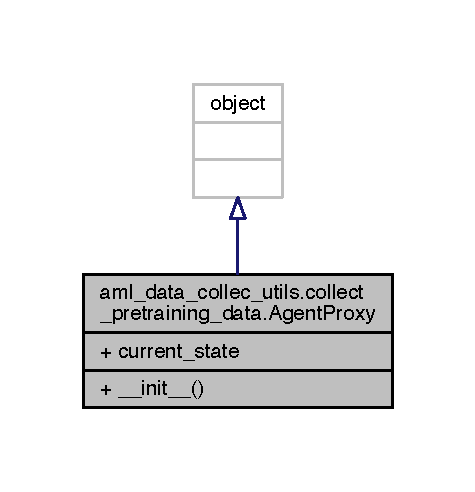
\includegraphics[width=224pt]{classaml__data__collec__utils_1_1collect__pretraining__data_1_1_agent_proxy__inherit__graph}
\end{center}
\end{figure}


Collaboration diagram for aml\-\_\-data\-\_\-collec\-\_\-utils.\-collect\-\_\-pretraining\-\_\-data.\-Agent\-Proxy\-:
\nopagebreak
\begin{figure}[H]
\begin{center}
\leavevmode
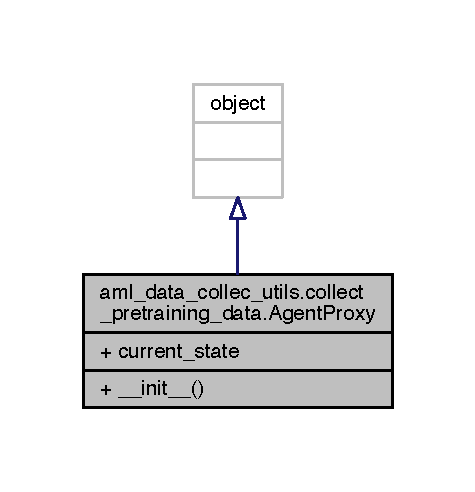
\includegraphics[width=224pt]{classaml__data__collec__utils_1_1collect__pretraining__data_1_1_agent_proxy__coll__graph}
\end{center}
\end{figure}
\subsection*{Public Member Functions}
\begin{DoxyCompactItemize}
\item 
\hypertarget{classaml__data__collec__utils_1_1collect__pretraining__data_1_1_agent_proxy_a0ba09dbbb1e176464aa07485f77cf9f9}{def {\bfseries \-\_\-\-\_\-init\-\_\-\-\_\-}}\label{classaml__data__collec__utils_1_1collect__pretraining__data_1_1_agent_proxy_a0ba09dbbb1e176464aa07485f77cf9f9}

\end{DoxyCompactItemize}
\subsection*{Public Attributes}
\begin{DoxyCompactItemize}
\item 
\hypertarget{classaml__data__collec__utils_1_1collect__pretraining__data_1_1_agent_proxy_aeb2225b6b78553e00dfa022cd7bafd49}{{\bfseries current\-\_\-state}}\label{classaml__data__collec__utils_1_1collect__pretraining__data_1_1_agent_proxy_aeb2225b6b78553e00dfa022cd7bafd49}

\end{DoxyCompactItemize}


The documentation for this class was generated from the following file\-:\begin{DoxyCompactItemize}
\item 
aml\-\_\-data\-\_\-collec\-\_\-utils/src/aml\-\_\-data\-\_\-collec\-\_\-utils/collect\-\_\-pretraining\-\_\-data.\-py\end{DoxyCompactItemize}

\hypertarget{classcamera__calib_1_1_baxter___eye___hand___calib}{}\section{camera\+\_\+calib.\+Baxter\+\_\+\+Eye\+\_\+\+Hand\+\_\+\+Calib Class Reference}
\label{classcamera__calib_1_1_baxter___eye___hand___calib}\index{camera\+\_\+calib.\+Baxter\+\_\+\+Eye\+\_\+\+Hand\+\_\+\+Calib@{camera\+\_\+calib.\+Baxter\+\_\+\+Eye\+\_\+\+Hand\+\_\+\+Calib}}


Collaboration diagram for camera\+\_\+calib.\+Baxter\+\_\+\+Eye\+\_\+\+Hand\+\_\+\+Calib\+:
\nopagebreak
\begin{figure}[H]
\begin{center}
\leavevmode
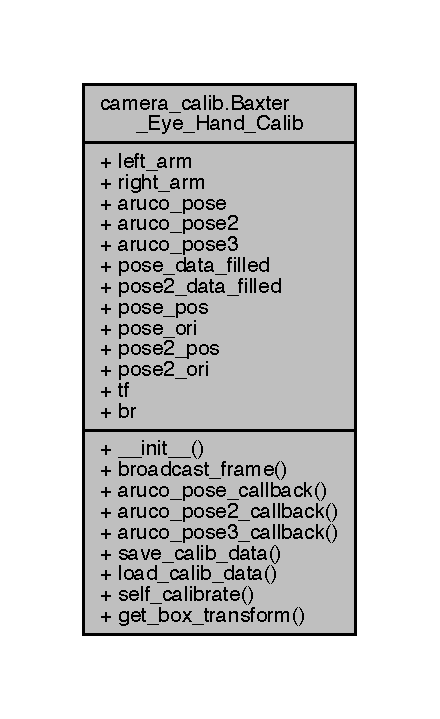
\includegraphics[width=211pt]{classcamera__calib_1_1_baxter___eye___hand___calib__coll__graph}
\end{center}
\end{figure}
\subsection*{Public Member Functions}
\begin{DoxyCompactItemize}
\item 
\hypertarget{classcamera__calib_1_1_baxter___eye___hand___calib_af3ebb65cba8f8de8553341c5403c58a7}{}\label{classcamera__calib_1_1_baxter___eye___hand___calib_af3ebb65cba8f8de8553341c5403c58a7} 
def {\bfseries \+\_\+\+\_\+init\+\_\+\+\_\+} (self)
\item 
\hypertarget{classcamera__calib_1_1_baxter___eye___hand___calib_a8e93d01429d7bb4c08223f39534c8ef7}{}\label{classcamera__calib_1_1_baxter___eye___hand___calib_a8e93d01429d7bb4c08223f39534c8ef7} 
def {\bfseries broadcast\+\_\+frame} (self, pt, rot, frame\+\_\+name=\char`\"{}marker\char`\"{})
\item 
\hypertarget{classcamera__calib_1_1_baxter___eye___hand___calib_aca31a7a1cfdca2ec3372486aaed8acec}{}\label{classcamera__calib_1_1_baxter___eye___hand___calib_aca31a7a1cfdca2ec3372486aaed8acec} 
def {\bfseries aruco\+\_\+pose\+\_\+callback} (self, data)
\item 
\hypertarget{classcamera__calib_1_1_baxter___eye___hand___calib_ade3d07a10851812da684461e39d88fef}{}\label{classcamera__calib_1_1_baxter___eye___hand___calib_ade3d07a10851812da684461e39d88fef} 
def {\bfseries aruco\+\_\+pose2\+\_\+callback} (self, data)
\item 
\hypertarget{classcamera__calib_1_1_baxter___eye___hand___calib_a059748e2d24c83d877effbf9dc093271}{}\label{classcamera__calib_1_1_baxter___eye___hand___calib_a059748e2d24c83d877effbf9dc093271} 
def {\bfseries aruco\+\_\+pose3\+\_\+callback} (self, data)
\item 
\hypertarget{classcamera__calib_1_1_baxter___eye___hand___calib_a86d89cb18fb192dd81e045415036457c}{}\label{classcamera__calib_1_1_baxter___eye___hand___calib_a86d89cb18fb192dd81e045415036457c} 
def {\bfseries save\+\_\+calib\+\_\+data} (self)
\item 
\hypertarget{classcamera__calib_1_1_baxter___eye___hand___calib_a5c601642e0efcaca54ac63417e0f824d}{}\label{classcamera__calib_1_1_baxter___eye___hand___calib_a5c601642e0efcaca54ac63417e0f824d} 
def {\bfseries load\+\_\+calib\+\_\+data} (self)
\item 
\hypertarget{classcamera__calib_1_1_baxter___eye___hand___calib_aeeb5e99b79b3c69dd13d5ac2f01708f6}{}\label{classcamera__calib_1_1_baxter___eye___hand___calib_aeeb5e99b79b3c69dd13d5ac2f01708f6} 
def {\bfseries self\+\_\+calibrate} (self)
\item 
\hypertarget{classcamera__calib_1_1_baxter___eye___hand___calib_ace15c3cc82853360ec6bddb2c89aaa27}{}\label{classcamera__calib_1_1_baxter___eye___hand___calib_ace15c3cc82853360ec6bddb2c89aaa27} 
def {\bfseries get\+\_\+box\+\_\+transform} (self)
\end{DoxyCompactItemize}
\subsection*{Public Attributes}
\begin{DoxyCompactItemize}
\item 
\hypertarget{classcamera__calib_1_1_baxter___eye___hand___calib_aa2a792295a271c8202bd39366c59eef7}{}\label{classcamera__calib_1_1_baxter___eye___hand___calib_aa2a792295a271c8202bd39366c59eef7} 
{\bfseries left\+\_\+arm}
\item 
\hypertarget{classcamera__calib_1_1_baxter___eye___hand___calib_a6e651fc54d9e6272c837783f473434e7}{}\label{classcamera__calib_1_1_baxter___eye___hand___calib_a6e651fc54d9e6272c837783f473434e7} 
{\bfseries right\+\_\+arm}
\item 
\hypertarget{classcamera__calib_1_1_baxter___eye___hand___calib_ac7c3bae776d3c8a1e4020d3c2b70ae79}{}\label{classcamera__calib_1_1_baxter___eye___hand___calib_ac7c3bae776d3c8a1e4020d3c2b70ae79} 
{\bfseries aruco\+\_\+pose}
\item 
\hypertarget{classcamera__calib_1_1_baxter___eye___hand___calib_aace16a5ef26f5ae5caa25e40f6c1c187}{}\label{classcamera__calib_1_1_baxter___eye___hand___calib_aace16a5ef26f5ae5caa25e40f6c1c187} 
{\bfseries aruco\+\_\+pose2}
\item 
\hypertarget{classcamera__calib_1_1_baxter___eye___hand___calib_ae672c226b1267cd55a720c00cc3b1fb9}{}\label{classcamera__calib_1_1_baxter___eye___hand___calib_ae672c226b1267cd55a720c00cc3b1fb9} 
{\bfseries aruco\+\_\+pose3}
\item 
\hypertarget{classcamera__calib_1_1_baxter___eye___hand___calib_ac1bc1c3e52000ed336c8b20266ee2276}{}\label{classcamera__calib_1_1_baxter___eye___hand___calib_ac1bc1c3e52000ed336c8b20266ee2276} 
{\bfseries pose\+\_\+data\+\_\+filled}
\item 
\hypertarget{classcamera__calib_1_1_baxter___eye___hand___calib_ac0e4523804fdf7c3165699ec28102bec}{}\label{classcamera__calib_1_1_baxter___eye___hand___calib_ac0e4523804fdf7c3165699ec28102bec} 
{\bfseries pose2\+\_\+data\+\_\+filled}
\item 
\hypertarget{classcamera__calib_1_1_baxter___eye___hand___calib_ab8e2acfb8ea62ab610a62fad3e9935d7}{}\label{classcamera__calib_1_1_baxter___eye___hand___calib_ab8e2acfb8ea62ab610a62fad3e9935d7} 
{\bfseries pose\+\_\+pos}
\item 
\hypertarget{classcamera__calib_1_1_baxter___eye___hand___calib_adf041f3f0bb402ea082b5c8c585c8ecd}{}\label{classcamera__calib_1_1_baxter___eye___hand___calib_adf041f3f0bb402ea082b5c8c585c8ecd} 
{\bfseries pose\+\_\+ori}
\item 
\hypertarget{classcamera__calib_1_1_baxter___eye___hand___calib_ae7be52d3c7dcec84c72263ba478d9836}{}\label{classcamera__calib_1_1_baxter___eye___hand___calib_ae7be52d3c7dcec84c72263ba478d9836} 
{\bfseries pose2\+\_\+pos}
\item 
\hypertarget{classcamera__calib_1_1_baxter___eye___hand___calib_ab4c5e265b75dbc426e02d079ef8f1030}{}\label{classcamera__calib_1_1_baxter___eye___hand___calib_ab4c5e265b75dbc426e02d079ef8f1030} 
{\bfseries pose2\+\_\+ori}
\item 
\hypertarget{classcamera__calib_1_1_baxter___eye___hand___calib_a43206bf881a79c98ddd86917efbf2239}{}\label{classcamera__calib_1_1_baxter___eye___hand___calib_a43206bf881a79c98ddd86917efbf2239} 
{\bfseries tf}
\item 
\hypertarget{classcamera__calib_1_1_baxter___eye___hand___calib_a55dcc04199f3a490cccf70ef66d467a0}{}\label{classcamera__calib_1_1_baxter___eye___hand___calib_a55dcc04199f3a490cccf70ef66d467a0} 
{\bfseries br}
\end{DoxyCompactItemize}


The documentation for this class was generated from the following file\+:\begin{DoxyCompactItemize}
\item 
aml\+\_\+calib/scripts/camera\+\_\+calib.\+py\end{DoxyCompactItemize}

\hypertarget{classaml__robot_1_1baxter__kinematics_1_1baxter__kinematics}{\section{aml\-\_\-robot.\-baxter\-\_\-kinematics.\-baxter\-\_\-kinematics Class Reference}
\label{classaml__robot_1_1baxter__kinematics_1_1baxter__kinematics}\index{aml\-\_\-robot.\-baxter\-\_\-kinematics.\-baxter\-\_\-kinematics@{aml\-\_\-robot.\-baxter\-\_\-kinematics.\-baxter\-\_\-kinematics}}
}


Inheritance diagram for aml\-\_\-robot.\-baxter\-\_\-kinematics.\-baxter\-\_\-kinematics\-:\nopagebreak
\begin{figure}[H]
\begin{center}
\leavevmode
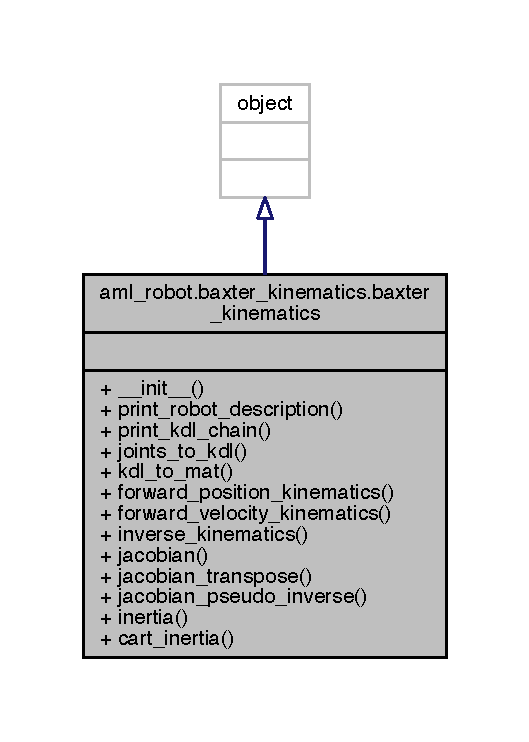
\includegraphics[width=252pt]{classaml__robot_1_1baxter__kinematics_1_1baxter__kinematics__inherit__graph}
\end{center}
\end{figure}


Collaboration diagram for aml\-\_\-robot.\-baxter\-\_\-kinematics.\-baxter\-\_\-kinematics\-:\nopagebreak
\begin{figure}[H]
\begin{center}
\leavevmode
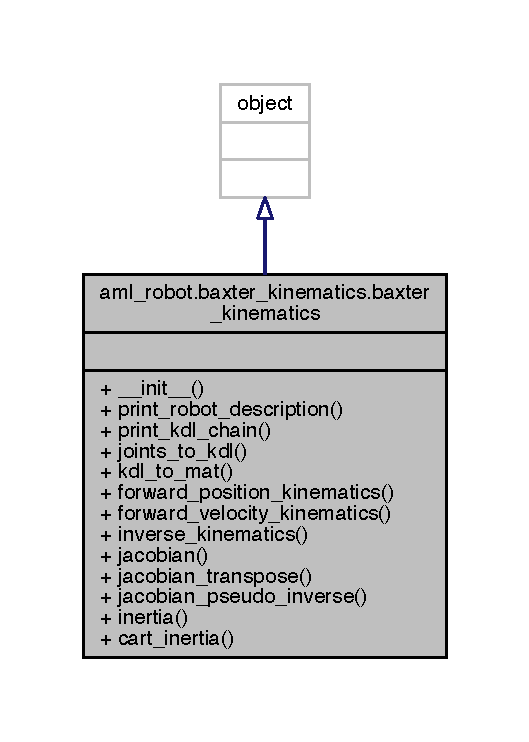
\includegraphics[width=252pt]{classaml__robot_1_1baxter__kinematics_1_1baxter__kinematics__coll__graph}
\end{center}
\end{figure}
\subsection*{Public Member Functions}
\begin{DoxyCompactItemize}
\item 
\hypertarget{classaml__robot_1_1baxter__kinematics_1_1baxter__kinematics_a6a642546348903ad83647e46b3997319}{def {\bfseries \-\_\-\-\_\-init\-\_\-\-\_\-}}\label{classaml__robot_1_1baxter__kinematics_1_1baxter__kinematics_a6a642546348903ad83647e46b3997319}

\item 
\hypertarget{classaml__robot_1_1baxter__kinematics_1_1baxter__kinematics_a5f20f5ed9f8e063544fe0f9269824d77}{def {\bfseries print\-\_\-robot\-\_\-description}}\label{classaml__robot_1_1baxter__kinematics_1_1baxter__kinematics_a5f20f5ed9f8e063544fe0f9269824d77}

\item 
\hypertarget{classaml__robot_1_1baxter__kinematics_1_1baxter__kinematics_a6505980cb91459683b46b4eb0ed5048f}{def {\bfseries print\-\_\-kdl\-\_\-chain}}\label{classaml__robot_1_1baxter__kinematics_1_1baxter__kinematics_a6505980cb91459683b46b4eb0ed5048f}

\item 
\hypertarget{classaml__robot_1_1baxter__kinematics_1_1baxter__kinematics_a5b33fe6f350f58a6b1eab83aa072d847}{def {\bfseries joints\-\_\-to\-\_\-kdl}}\label{classaml__robot_1_1baxter__kinematics_1_1baxter__kinematics_a5b33fe6f350f58a6b1eab83aa072d847}

\item 
\hypertarget{classaml__robot_1_1baxter__kinematics_1_1baxter__kinematics_a4b961c3b58138f41aa1b0f4f34da7e83}{def {\bfseries kdl\-\_\-to\-\_\-mat}}\label{classaml__robot_1_1baxter__kinematics_1_1baxter__kinematics_a4b961c3b58138f41aa1b0f4f34da7e83}

\item 
\hypertarget{classaml__robot_1_1baxter__kinematics_1_1baxter__kinematics_a4c3c9043ae935f5ae5c4bb5806532071}{def {\bfseries forward\-\_\-position\-\_\-kinematics}}\label{classaml__robot_1_1baxter__kinematics_1_1baxter__kinematics_a4c3c9043ae935f5ae5c4bb5806532071}

\item 
\hypertarget{classaml__robot_1_1baxter__kinematics_1_1baxter__kinematics_aca2eef593f0f9e6095c13153401eb948}{def {\bfseries forward\-\_\-velocity\-\_\-kinematics}}\label{classaml__robot_1_1baxter__kinematics_1_1baxter__kinematics_aca2eef593f0f9e6095c13153401eb948}

\item 
\hypertarget{classaml__robot_1_1baxter__kinematics_1_1baxter__kinematics_a5eaca30766683990b213182527cb3813}{def {\bfseries inverse\-\_\-kinematics}}\label{classaml__robot_1_1baxter__kinematics_1_1baxter__kinematics_a5eaca30766683990b213182527cb3813}

\item 
\hypertarget{classaml__robot_1_1baxter__kinematics_1_1baxter__kinematics_a307997661ec9ef26ae4a74bda67a3352}{def {\bfseries jacobian}}\label{classaml__robot_1_1baxter__kinematics_1_1baxter__kinematics_a307997661ec9ef26ae4a74bda67a3352}

\item 
\hypertarget{classaml__robot_1_1baxter__kinematics_1_1baxter__kinematics_a421d5a7383a8b88e7b03efc469f30098}{def {\bfseries jacobian\-\_\-transpose}}\label{classaml__robot_1_1baxter__kinematics_1_1baxter__kinematics_a421d5a7383a8b88e7b03efc469f30098}

\item 
\hypertarget{classaml__robot_1_1baxter__kinematics_1_1baxter__kinematics_ad70f0257064b8a85ee6537e2187822d8}{def {\bfseries jacobian\-\_\-pseudo\-\_\-inverse}}\label{classaml__robot_1_1baxter__kinematics_1_1baxter__kinematics_ad70f0257064b8a85ee6537e2187822d8}

\item 
\hypertarget{classaml__robot_1_1baxter__kinematics_1_1baxter__kinematics_a7fd0653ad6b2012a933822f98901ccce}{def {\bfseries inertia}}\label{classaml__robot_1_1baxter__kinematics_1_1baxter__kinematics_a7fd0653ad6b2012a933822f98901ccce}

\item 
\hypertarget{classaml__robot_1_1baxter__kinematics_1_1baxter__kinematics_af243bf47f45355fb5e71a23ed8b21d28}{def {\bfseries cart\-\_\-inertia}}\label{classaml__robot_1_1baxter__kinematics_1_1baxter__kinematics_af243bf47f45355fb5e71a23ed8b21d28}

\end{DoxyCompactItemize}


\subsection{Detailed Description}
\begin{DoxyVerb}Baxter Kinematics with PyKDL
\end{DoxyVerb}
 

The documentation for this class was generated from the following file\-:\begin{DoxyCompactItemize}
\item 
aml\-\_\-robot/src/aml\-\_\-robot/baxter\-\_\-kinematics.\-py\end{DoxyCompactItemize}

\hypertarget{classaml__robot_1_1baxter__robot_1_1_baxter_arm}{}\section{aml\+\_\+robot.\+baxter\+\_\+robot.\+Baxter\+Arm Class Reference}
\label{classaml__robot_1_1baxter__robot_1_1_baxter_arm}\index{aml\+\_\+robot.\+baxter\+\_\+robot.\+Baxter\+Arm@{aml\+\_\+robot.\+baxter\+\_\+robot.\+Baxter\+Arm}}


Inheritance diagram for aml\+\_\+robot.\+baxter\+\_\+robot.\+Baxter\+Arm\+:
\nopagebreak
\begin{figure}[H]
\begin{center}
\leavevmode
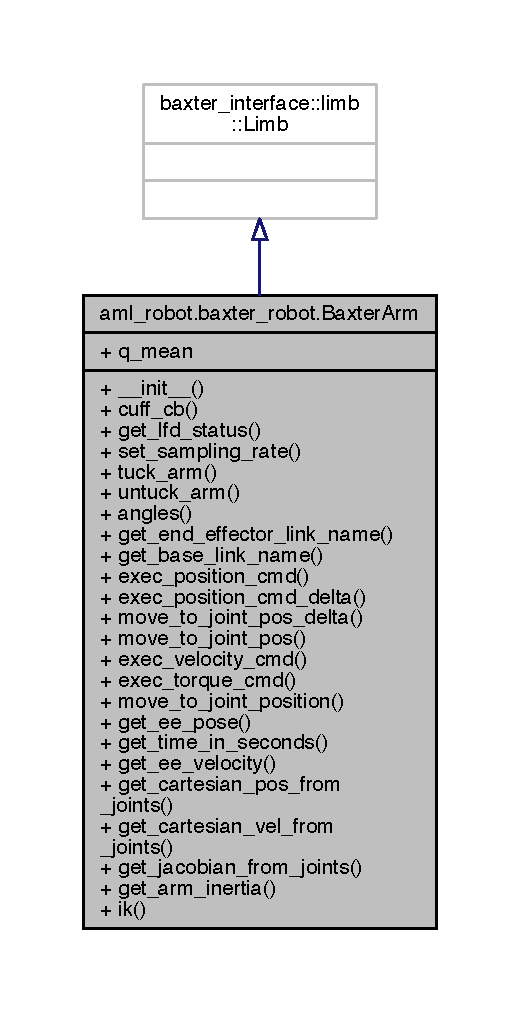
\includegraphics[width=249pt]{classaml__robot_1_1baxter__robot_1_1_baxter_arm__inherit__graph}
\end{center}
\end{figure}


Collaboration diagram for aml\+\_\+robot.\+baxter\+\_\+robot.\+Baxter\+Arm\+:
\nopagebreak
\begin{figure}[H]
\begin{center}
\leavevmode
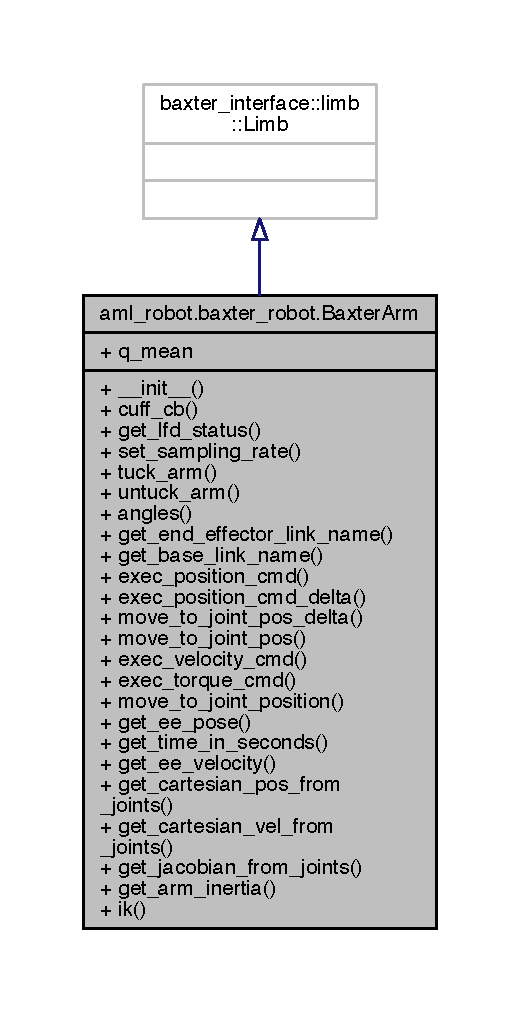
\includegraphics[width=249pt]{classaml__robot_1_1baxter__robot_1_1_baxter_arm__coll__graph}
\end{center}
\end{figure}
\subsection*{Public Member Functions}
\begin{DoxyCompactItemize}
\item 
\hypertarget{classaml__robot_1_1baxter__robot_1_1_baxter_arm_a72a5c161c29bd536c6a8727d3138643a}{}\label{classaml__robot_1_1baxter__robot_1_1_baxter_arm_a72a5c161c29bd536c6a8727d3138643a} 
def {\bfseries \+\_\+\+\_\+init\+\_\+\+\_\+} (self, limb, on\+\_\+state\+\_\+callback=None)
\item 
\hypertarget{classaml__robot_1_1baxter__robot_1_1_baxter_arm_ab8c5985c2c013d2da84e7415f2480f35}{}\label{classaml__robot_1_1baxter__robot_1_1_baxter_arm_ab8c5985c2c013d2da84e7415f2480f35} 
def {\bfseries cuff\+\_\+cb} (self, value)
\item 
\hypertarget{classaml__robot_1_1baxter__robot_1_1_baxter_arm_a08034a334645d8504b391a313add1cc7}{}\label{classaml__robot_1_1baxter__robot_1_1_baxter_arm_a08034a334645d8504b391a313add1cc7} 
def {\bfseries get\+\_\+lfd\+\_\+status} (self)
\item 
\hypertarget{classaml__robot_1_1baxter__robot_1_1_baxter_arm_a1f1b2c10d8e309c0cce60a971f5355b4}{}\label{classaml__robot_1_1baxter__robot_1_1_baxter_arm_a1f1b2c10d8e309c0cce60a971f5355b4} 
def {\bfseries set\+\_\+sampling\+\_\+rate} (self, sampling\+\_\+rate=100)
\item 
\hypertarget{classaml__robot_1_1baxter__robot_1_1_baxter_arm_add8768944b81542e122c676f2b38c075}{}\label{classaml__robot_1_1baxter__robot_1_1_baxter_arm_add8768944b81542e122c676f2b38c075} 
def {\bfseries tuck\+\_\+arm} (self)
\item 
\hypertarget{classaml__robot_1_1baxter__robot_1_1_baxter_arm_af3664aaae25213bf3930c821cbf68432}{}\label{classaml__robot_1_1baxter__robot_1_1_baxter_arm_af3664aaae25213bf3930c821cbf68432} 
def {\bfseries untuck\+\_\+arm} (self)
\item 
\hypertarget{classaml__robot_1_1baxter__robot_1_1_baxter_arm_a0434abfd5899e880a6856444ccc9ecae}{}\label{classaml__robot_1_1baxter__robot_1_1_baxter_arm_a0434abfd5899e880a6856444ccc9ecae} 
def {\bfseries angles} (self)
\item 
\hypertarget{classaml__robot_1_1baxter__robot_1_1_baxter_arm_a40dc93e2269ea57aec71457431984bc0}{}\label{classaml__robot_1_1baxter__robot_1_1_baxter_arm_a40dc93e2269ea57aec71457431984bc0} 
def {\bfseries get\+\_\+end\+\_\+effector\+\_\+link\+\_\+name} (self)
\item 
\hypertarget{classaml__robot_1_1baxter__robot_1_1_baxter_arm_a3d7c1dd8493d6ed1255e856db43e4d9c}{}\label{classaml__robot_1_1baxter__robot_1_1_baxter_arm_a3d7c1dd8493d6ed1255e856db43e4d9c} 
def {\bfseries get\+\_\+base\+\_\+link\+\_\+name} (self)
\item 
\hypertarget{classaml__robot_1_1baxter__robot_1_1_baxter_arm_aa8fb038222939675c5038f546d0e2627}{}\label{classaml__robot_1_1baxter__robot_1_1_baxter_arm_aa8fb038222939675c5038f546d0e2627} 
def {\bfseries exec\+\_\+position\+\_\+cmd} (self, cmd)
\item 
\hypertarget{classaml__robot_1_1baxter__robot_1_1_baxter_arm_a7231f60bcd22ea25ee84d5c3269e82ae}{}\label{classaml__robot_1_1baxter__robot_1_1_baxter_arm_a7231f60bcd22ea25ee84d5c3269e82ae} 
def {\bfseries exec\+\_\+position\+\_\+cmd\+\_\+delta} (self, cmd)
\item 
\hypertarget{classaml__robot_1_1baxter__robot_1_1_baxter_arm_ad4c0f6a22d0cb23f411d50e8f661bcbb}{}\label{classaml__robot_1_1baxter__robot_1_1_baxter_arm_ad4c0f6a22d0cb23f411d50e8f661bcbb} 
def {\bfseries move\+\_\+to\+\_\+joint\+\_\+pos\+\_\+delta} (self, cmd)
\item 
\hypertarget{classaml__robot_1_1baxter__robot_1_1_baxter_arm_a93f87a8500f9e0bfce6be75e41e3ac17}{}\label{classaml__robot_1_1baxter__robot_1_1_baxter_arm_a93f87a8500f9e0bfce6be75e41e3ac17} 
def {\bfseries move\+\_\+to\+\_\+joint\+\_\+pos} (self, cmd)
\item 
\hypertarget{classaml__robot_1_1baxter__robot_1_1_baxter_arm_a3b5cb3d6c651c72bfe9ffd80c867f8f7}{}\label{classaml__robot_1_1baxter__robot_1_1_baxter_arm_a3b5cb3d6c651c72bfe9ffd80c867f8f7} 
def {\bfseries exec\+\_\+velocity\+\_\+cmd} (self, cmd)
\item 
\hypertarget{classaml__robot_1_1baxter__robot_1_1_baxter_arm_aed8c9accc1f637677e4d64583b63d107}{}\label{classaml__robot_1_1baxter__robot_1_1_baxter_arm_aed8c9accc1f637677e4d64583b63d107} 
def {\bfseries exec\+\_\+torque\+\_\+cmd} (self, cmd)
\item 
\hypertarget{classaml__robot_1_1baxter__robot_1_1_baxter_arm_afddcdfa0cafe258cf7f432e7878bc687}{}\label{classaml__robot_1_1baxter__robot_1_1_baxter_arm_afddcdfa0cafe258cf7f432e7878bc687} 
def {\bfseries move\+\_\+to\+\_\+joint\+\_\+position} (self, joint\+\_\+angles)
\item 
\hypertarget{classaml__robot_1_1baxter__robot_1_1_baxter_arm_ac353cdab96098923a40efd30f17f4e7a}{}\label{classaml__robot_1_1baxter__robot_1_1_baxter_arm_ac353cdab96098923a40efd30f17f4e7a} 
def {\bfseries get\+\_\+ee\+\_\+pose} (self)
\item 
\hypertarget{classaml__robot_1_1baxter__robot_1_1_baxter_arm_a9dcc207d5f7703f7f9f69bb54c1ee7b3}{}\label{classaml__robot_1_1baxter__robot_1_1_baxter_arm_a9dcc207d5f7703f7f9f69bb54c1ee7b3} 
def {\bfseries get\+\_\+time\+\_\+in\+\_\+seconds} (self)
\item 
\hypertarget{classaml__robot_1_1baxter__robot_1_1_baxter_arm_a411092f179a7420d38625063c27b237e}{}\label{classaml__robot_1_1baxter__robot_1_1_baxter_arm_a411092f179a7420d38625063c27b237e} 
def {\bfseries get\+\_\+ee\+\_\+velocity} (self, real\+\_\+robot=True)
\item 
\hypertarget{classaml__robot_1_1baxter__robot_1_1_baxter_arm_a9ce9c74c445092b5f9bd26793366c8de}{}\label{classaml__robot_1_1baxter__robot_1_1_baxter_arm_a9ce9c74c445092b5f9bd26793366c8de} 
def {\bfseries get\+\_\+cartesian\+\_\+pos\+\_\+from\+\_\+joints} (self, joint\+\_\+angles=None)
\item 
\hypertarget{classaml__robot_1_1baxter__robot_1_1_baxter_arm_a5d42a91ca13fc1776997909afb999d8f}{}\label{classaml__robot_1_1baxter__robot_1_1_baxter_arm_a5d42a91ca13fc1776997909afb999d8f} 
def {\bfseries get\+\_\+cartesian\+\_\+vel\+\_\+from\+\_\+joints} (self, joint\+\_\+angles=None)
\item 
\hypertarget{classaml__robot_1_1baxter__robot_1_1_baxter_arm_a05c9ee1fe630edbcdc34249bb0c613b3}{}\label{classaml__robot_1_1baxter__robot_1_1_baxter_arm_a05c9ee1fe630edbcdc34249bb0c613b3} 
def {\bfseries get\+\_\+jacobian\+\_\+from\+\_\+joints} (self, joint\+\_\+angles=None)
\item 
\hypertarget{classaml__robot_1_1baxter__robot_1_1_baxter_arm_ae3980ca9408490d07b4460e6d7fc2eb2}{}\label{classaml__robot_1_1baxter__robot_1_1_baxter_arm_ae3980ca9408490d07b4460e6d7fc2eb2} 
def {\bfseries get\+\_\+arm\+\_\+inertia} (self, joint\+\_\+angles=None)
\item 
\hypertarget{classaml__robot_1_1baxter__robot_1_1_baxter_arm_a5ce4a9920b76e223e375755faaef7cf5}{}\label{classaml__robot_1_1baxter__robot_1_1_baxter_arm_a5ce4a9920b76e223e375755faaef7cf5} 
def {\bfseries ik} (self, pos, ori=None)
\end{DoxyCompactItemize}
\subsection*{Public Attributes}
\begin{DoxyCompactItemize}
\item 
\hypertarget{classaml__robot_1_1baxter__robot_1_1_baxter_arm_adf4365cfefdb2632a538a3f225023aa7}{}\label{classaml__robot_1_1baxter__robot_1_1_baxter_arm_adf4365cfefdb2632a538a3f225023aa7} 
{\bfseries q\+\_\+mean}
\end{DoxyCompactItemize}


The documentation for this class was generated from the following file\+:\begin{DoxyCompactItemize}
\item 
aml\+\_\+robot/src/aml\+\_\+robot/baxter\+\_\+robot.\+py\end{DoxyCompactItemize}

\hypertarget{classaml__robot_1_1baxter__robot_1_1_baxter_button_status}{}\section{aml\+\_\+robot.\+baxter\+\_\+robot.\+Baxter\+Button\+Status Class Reference}
\label{classaml__robot_1_1baxter__robot_1_1_baxter_button_status}\index{aml\+\_\+robot.\+baxter\+\_\+robot.\+Baxter\+Button\+Status@{aml\+\_\+robot.\+baxter\+\_\+robot.\+Baxter\+Button\+Status}}


Collaboration diagram for aml\+\_\+robot.\+baxter\+\_\+robot.\+Baxter\+Button\+Status\+:
\nopagebreak
\begin{figure}[H]
\begin{center}
\leavevmode
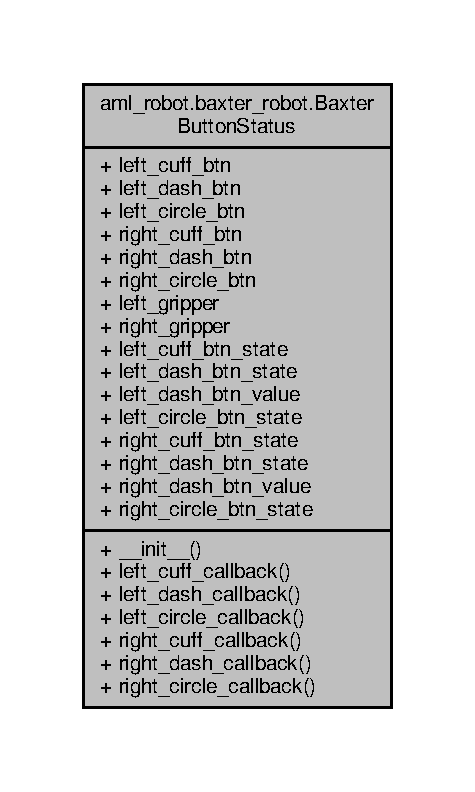
\includegraphics[width=231pt]{classaml__robot_1_1baxter__robot_1_1_baxter_button_status__coll__graph}
\end{center}
\end{figure}
\subsection*{Public Member Functions}
\begin{DoxyCompactItemize}
\item 
\hypertarget{classaml__robot_1_1baxter__robot_1_1_baxter_button_status_a867cbab0efc9f033f193484b7a6ee7d9}{}\label{classaml__robot_1_1baxter__robot_1_1_baxter_button_status_a867cbab0efc9f033f193484b7a6ee7d9} 
def {\bfseries \+\_\+\+\_\+init\+\_\+\+\_\+} (self)
\item 
\hypertarget{classaml__robot_1_1baxter__robot_1_1_baxter_button_status_a0be7e8628a069cee960ba4f84a1fba42}{}\label{classaml__robot_1_1baxter__robot_1_1_baxter_button_status_a0be7e8628a069cee960ba4f84a1fba42} 
def {\bfseries left\+\_\+cuff\+\_\+callback} (self, value)
\item 
\hypertarget{classaml__robot_1_1baxter__robot_1_1_baxter_button_status_a0c7539db9445b453a0eac9e24d402b89}{}\label{classaml__robot_1_1baxter__robot_1_1_baxter_button_status_a0c7539db9445b453a0eac9e24d402b89} 
def {\bfseries left\+\_\+dash\+\_\+callback} (self, value)
\item 
\hypertarget{classaml__robot_1_1baxter__robot_1_1_baxter_button_status_a2a5e12090c441e098b287596bac9b2e9}{}\label{classaml__robot_1_1baxter__robot_1_1_baxter_button_status_a2a5e12090c441e098b287596bac9b2e9} 
def {\bfseries left\+\_\+circle\+\_\+callback} (self, value)
\item 
\hypertarget{classaml__robot_1_1baxter__robot_1_1_baxter_button_status_aea7f6e2c3cb75cc764898bacdf24adad}{}\label{classaml__robot_1_1baxter__robot_1_1_baxter_button_status_aea7f6e2c3cb75cc764898bacdf24adad} 
def {\bfseries right\+\_\+cuff\+\_\+callback} (self, value)
\item 
\hypertarget{classaml__robot_1_1baxter__robot_1_1_baxter_button_status_a9ebd13514e6d978c3a022b99f56d0d2d}{}\label{classaml__robot_1_1baxter__robot_1_1_baxter_button_status_a9ebd13514e6d978c3a022b99f56d0d2d} 
def {\bfseries right\+\_\+dash\+\_\+callback} (self, value)
\item 
\hypertarget{classaml__robot_1_1baxter__robot_1_1_baxter_button_status_a80e8aebd2bf7ceb32d63bade6e078eff}{}\label{classaml__robot_1_1baxter__robot_1_1_baxter_button_status_a80e8aebd2bf7ceb32d63bade6e078eff} 
def {\bfseries right\+\_\+circle\+\_\+callback} (self, value)
\end{DoxyCompactItemize}
\subsection*{Public Attributes}
\begin{DoxyCompactItemize}
\item 
\hypertarget{classaml__robot_1_1baxter__robot_1_1_baxter_button_status_a04619f9d86af362ba45b652a30f75186}{}\label{classaml__robot_1_1baxter__robot_1_1_baxter_button_status_a04619f9d86af362ba45b652a30f75186} 
{\bfseries left\+\_\+cuff\+\_\+btn}
\item 
\hypertarget{classaml__robot_1_1baxter__robot_1_1_baxter_button_status_a8bf46c388908af610775a7853f12db6b}{}\label{classaml__robot_1_1baxter__robot_1_1_baxter_button_status_a8bf46c388908af610775a7853f12db6b} 
{\bfseries left\+\_\+dash\+\_\+btn}
\item 
\hypertarget{classaml__robot_1_1baxter__robot_1_1_baxter_button_status_aafc55b8a39cd12b8b916c1f9e4e101cb}{}\label{classaml__robot_1_1baxter__robot_1_1_baxter_button_status_aafc55b8a39cd12b8b916c1f9e4e101cb} 
{\bfseries left\+\_\+circle\+\_\+btn}
\item 
\hypertarget{classaml__robot_1_1baxter__robot_1_1_baxter_button_status_a96d1d159449f8937e2c8605ffb359e26}{}\label{classaml__robot_1_1baxter__robot_1_1_baxter_button_status_a96d1d159449f8937e2c8605ffb359e26} 
{\bfseries right\+\_\+cuff\+\_\+btn}
\item 
\hypertarget{classaml__robot_1_1baxter__robot_1_1_baxter_button_status_a20e886d155229257692984a1fc790216}{}\label{classaml__robot_1_1baxter__robot_1_1_baxter_button_status_a20e886d155229257692984a1fc790216} 
{\bfseries right\+\_\+dash\+\_\+btn}
\item 
\hypertarget{classaml__robot_1_1baxter__robot_1_1_baxter_button_status_af554ad16b5a28ab857cdc6c1d0e92ad8}{}\label{classaml__robot_1_1baxter__robot_1_1_baxter_button_status_af554ad16b5a28ab857cdc6c1d0e92ad8} 
{\bfseries right\+\_\+circle\+\_\+btn}
\item 
\hypertarget{classaml__robot_1_1baxter__robot_1_1_baxter_button_status_a1c2a8b264d928929fa9cad5d97bdc817}{}\label{classaml__robot_1_1baxter__robot_1_1_baxter_button_status_a1c2a8b264d928929fa9cad5d97bdc817} 
{\bfseries left\+\_\+gripper}
\item 
\hypertarget{classaml__robot_1_1baxter__robot_1_1_baxter_button_status_a1dd2e91ddd93d9c40dc8e7f83926d908}{}\label{classaml__robot_1_1baxter__robot_1_1_baxter_button_status_a1dd2e91ddd93d9c40dc8e7f83926d908} 
{\bfseries right\+\_\+gripper}
\item 
\hypertarget{classaml__robot_1_1baxter__robot_1_1_baxter_button_status_a3d147c0e2ab38474d2cb2d2cb358e9c6}{}\label{classaml__robot_1_1baxter__robot_1_1_baxter_button_status_a3d147c0e2ab38474d2cb2d2cb358e9c6} 
{\bfseries left\+\_\+cuff\+\_\+btn\+\_\+state}
\item 
\hypertarget{classaml__robot_1_1baxter__robot_1_1_baxter_button_status_a9858defbdfd1953111bc032a679dfbf6}{}\label{classaml__robot_1_1baxter__robot_1_1_baxter_button_status_a9858defbdfd1953111bc032a679dfbf6} 
{\bfseries left\+\_\+dash\+\_\+btn\+\_\+state}
\item 
\hypertarget{classaml__robot_1_1baxter__robot_1_1_baxter_button_status_ac4505635cb0c3096d50145a00aa996e1}{}\label{classaml__robot_1_1baxter__robot_1_1_baxter_button_status_ac4505635cb0c3096d50145a00aa996e1} 
{\bfseries left\+\_\+dash\+\_\+btn\+\_\+value}
\item 
\hypertarget{classaml__robot_1_1baxter__robot_1_1_baxter_button_status_a2cf8425649007e50335a7eab640138bd}{}\label{classaml__robot_1_1baxter__robot_1_1_baxter_button_status_a2cf8425649007e50335a7eab640138bd} 
{\bfseries left\+\_\+circle\+\_\+btn\+\_\+state}
\item 
\hypertarget{classaml__robot_1_1baxter__robot_1_1_baxter_button_status_a0b2de8e8474d9e9217024692b425a0b4}{}\label{classaml__robot_1_1baxter__robot_1_1_baxter_button_status_a0b2de8e8474d9e9217024692b425a0b4} 
{\bfseries right\+\_\+cuff\+\_\+btn\+\_\+state}
\item 
\hypertarget{classaml__robot_1_1baxter__robot_1_1_baxter_button_status_a99abdcffd19c44a10cb1f4a875adbb2d}{}\label{classaml__robot_1_1baxter__robot_1_1_baxter_button_status_a99abdcffd19c44a10cb1f4a875adbb2d} 
{\bfseries right\+\_\+dash\+\_\+btn\+\_\+state}
\item 
\hypertarget{classaml__robot_1_1baxter__robot_1_1_baxter_button_status_a990924b4c4d0b7f05b7fc909b3b7cc2f}{}\label{classaml__robot_1_1baxter__robot_1_1_baxter_button_status_a990924b4c4d0b7f05b7fc909b3b7cc2f} 
{\bfseries right\+\_\+dash\+\_\+btn\+\_\+value}
\item 
\hypertarget{classaml__robot_1_1baxter__robot_1_1_baxter_button_status_a6b266aa0af869f160bd2654e6fde6756}{}\label{classaml__robot_1_1baxter__robot_1_1_baxter_button_status_a6b266aa0af869f160bd2654e6fde6756} 
{\bfseries right\+\_\+circle\+\_\+btn\+\_\+state}
\end{DoxyCompactItemize}


The documentation for this class was generated from the following file\+:\begin{DoxyCompactItemize}
\item 
aml\+\_\+robot/src/aml\+\_\+robot/baxter\+\_\+robot.\+py\end{DoxyCompactItemize}

\hypertarget{classaml__perception_1_1camera__sensor_1_1_camera_sensor}{\section{aml\-\_\-perception.\-camera\-\_\-sensor.\-Camera\-Sensor Class Reference}
\label{classaml__perception_1_1camera__sensor_1_1_camera_sensor}\index{aml\-\_\-perception.\-camera\-\_\-sensor.\-Camera\-Sensor@{aml\-\_\-perception.\-camera\-\_\-sensor.\-Camera\-Sensor}}
}


Inheritance diagram for aml\-\_\-perception.\-camera\-\_\-sensor.\-Camera\-Sensor\-:
\nopagebreak
\begin{figure}[H]
\begin{center}
\leavevmode
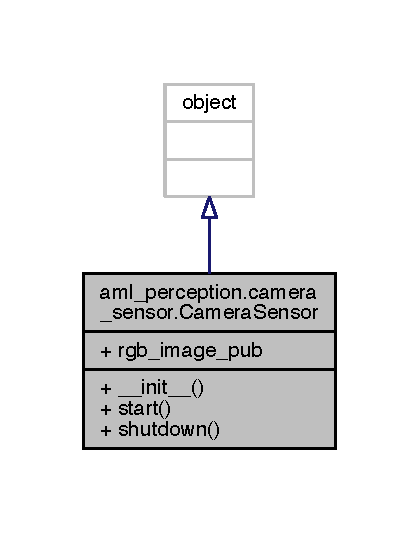
\includegraphics[width=198pt]{classaml__perception_1_1camera__sensor_1_1_camera_sensor__inherit__graph}
\end{center}
\end{figure}


Collaboration diagram for aml\-\_\-perception.\-camera\-\_\-sensor.\-Camera\-Sensor\-:
\nopagebreak
\begin{figure}[H]
\begin{center}
\leavevmode
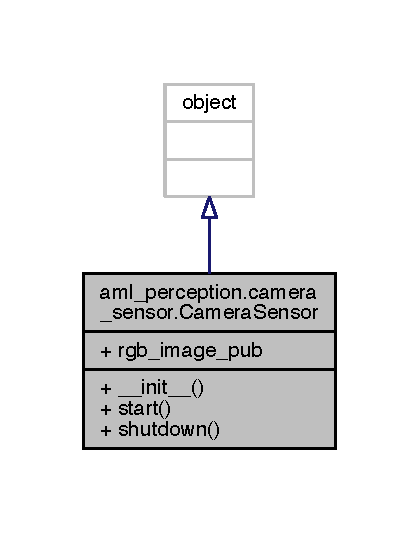
\includegraphics[width=198pt]{classaml__perception_1_1camera__sensor_1_1_camera_sensor__coll__graph}
\end{center}
\end{figure}
\subsection*{Public Member Functions}
\begin{DoxyCompactItemize}
\item 
\hypertarget{classaml__perception_1_1camera__sensor_1_1_camera_sensor_a21adf5c3740d47e8fb55c932e924618d}{def {\bfseries \-\_\-\-\_\-init\-\_\-\-\_\-}}\label{classaml__perception_1_1camera__sensor_1_1_camera_sensor_a21adf5c3740d47e8fb55c932e924618d}

\item 
\hypertarget{classaml__perception_1_1camera__sensor_1_1_camera_sensor_a08a06c82a0528c0462a49ec93db4dc0b}{def {\bfseries start}}\label{classaml__perception_1_1camera__sensor_1_1_camera_sensor_a08a06c82a0528c0462a49ec93db4dc0b}

\item 
\hypertarget{classaml__perception_1_1camera__sensor_1_1_camera_sensor_a95227671ed4cf14c09493d81bc619ea7}{def {\bfseries shutdown}}\label{classaml__perception_1_1camera__sensor_1_1_camera_sensor_a95227671ed4cf14c09493d81bc619ea7}

\item 
\hypertarget{classaml__perception_1_1camera__sensor_1_1_camera_sensor_adfbd28ea71c000f8ea5fed25868fb15f}{def {\bfseries set\-\_\-intrinsics}}\label{classaml__perception_1_1camera__sensor_1_1_camera_sensor_adfbd28ea71c000f8ea5fed25868fb15f}

\item 
\hypertarget{classaml__perception_1_1camera__sensor_1_1_camera_sensor_a57e0a5307a84544f0c0c5f8f1c0bc86b}{def {\bfseries intrinsics}}\label{classaml__perception_1_1camera__sensor_1_1_camera_sensor_a57e0a5307a84544f0c0c5f8f1c0bc86b}

\item 
\hypertarget{classaml__perception_1_1camera__sensor_1_1_camera_sensor_a0a599df52837dc5fc2debac009cbab99}{def {\bfseries rgb\-\_\-image}}\label{classaml__perception_1_1camera__sensor_1_1_camera_sensor_a0a599df52837dc5fc2debac009cbab99}

\item 
\hypertarget{classaml__perception_1_1camera__sensor_1_1_camera_sensor_ad77338064fe84b1932656006fdf5f366}{def {\bfseries depth\-\_\-image}}\label{classaml__perception_1_1camera__sensor_1_1_camera_sensor_ad77338064fe84b1932656006fdf5f366}

\item 
\hypertarget{classaml__perception_1_1camera__sensor_1_1_camera_sensor_abcd2dd8b9c56b814fccc4ae487835962}{def {\bfseries cloud}}\label{classaml__perception_1_1camera__sensor_1_1_camera_sensor_abcd2dd8b9c56b814fccc4ae487835962}

\item 
def \hyperlink{classaml__perception_1_1camera__sensor_1_1_camera_sensor_aa13c3fd9edecf042fb0a63daa1b2fc9a}{deproject}
\item 
def \hyperlink{classaml__perception_1_1camera__sensor_1_1_camera_sensor_a12f9efec439335da2874a9be29c63271}{project}
\end{DoxyCompactItemize}


\subsection{Member Function Documentation}
\hypertarget{classaml__perception_1_1camera__sensor_1_1_camera_sensor_aa13c3fd9edecf042fb0a63daa1b2fc9a}{\index{aml\-\_\-perception\-::camera\-\_\-sensor\-::\-Camera\-Sensor@{aml\-\_\-perception\-::camera\-\_\-sensor\-::\-Camera\-Sensor}!deproject@{deproject}}
\index{deproject@{deproject}!aml_perception::camera_sensor::CameraSensor@{aml\-\_\-perception\-::camera\-\_\-sensor\-::\-Camera\-Sensor}}
\subsubsection[{deproject}]{\setlength{\rightskip}{0pt plus 5cm}def aml\-\_\-perception.\-camera\-\_\-sensor.\-Camera\-Sensor.\-deproject (
\begin{DoxyParamCaption}
\item[{}]{self, }
\item[{}]{depth\-\_\-image}
\end{DoxyParamCaption}
)}}\label{classaml__perception_1_1camera__sensor_1_1_camera_sensor_aa13c3fd9edecf042fb0a63daa1b2fc9a}
\begin{DoxyVerb}Deprojects a depth image (2D numpy float array) into a point cloud
Params:

depth_image: (HxW numpy array of floats) 2D depth image to project
Returns:
3xN numpy float array of 3D points
\end{DoxyVerb}
 \hypertarget{classaml__perception_1_1camera__sensor_1_1_camera_sensor_a12f9efec439335da2874a9be29c63271}{\index{aml\-\_\-perception\-::camera\-\_\-sensor\-::\-Camera\-Sensor@{aml\-\_\-perception\-::camera\-\_\-sensor\-::\-Camera\-Sensor}!project@{project}}
\index{project@{project}!aml_perception::camera_sensor::CameraSensor@{aml\-\_\-perception\-::camera\-\_\-sensor\-::\-Camera\-Sensor}}
\subsubsection[{project}]{\setlength{\rightskip}{0pt plus 5cm}def aml\-\_\-perception.\-camera\-\_\-sensor.\-Camera\-Sensor.\-project (
\begin{DoxyParamCaption}
\item[{}]{self, }
\item[{}]{points}
\end{DoxyParamCaption}
)}}\label{classaml__perception_1_1camera__sensor_1_1_camera_sensor_a12f9efec439335da2874a9be29c63271}
\begin{DoxyVerb}Projects a set of points into the camera given by these parameters

Params:
points: (3xN numpy array of floats) 3D points to project
Returns:
2xN numpy float array of 2D image coordinates
1xN binary numpy array indicating whether or not point projected outside of image
\end{DoxyVerb}
 

The documentation for this class was generated from the following file\-:\begin{DoxyCompactItemize}
\item 
aml\-\_\-perception/src/aml\-\_\-perception/camera\-\_\-sensor.\-py\end{DoxyCompactItemize}

\hypertarget{classaml__ctrl_1_1classical__controller_1_1_classical_controller}{}\section{aml\+\_\+ctrl.\+classical\+\_\+controller.\+Classical\+Controller Class Reference}
\label{classaml__ctrl_1_1classical__controller_1_1_classical_controller}\index{aml\+\_\+ctrl.\+classical\+\_\+controller.\+Classical\+Controller@{aml\+\_\+ctrl.\+classical\+\_\+controller.\+Classical\+Controller}}


Inheritance diagram for aml\+\_\+ctrl.\+classical\+\_\+controller.\+Classical\+Controller\+:
\nopagebreak
\begin{figure}[H]
\begin{center}
\leavevmode
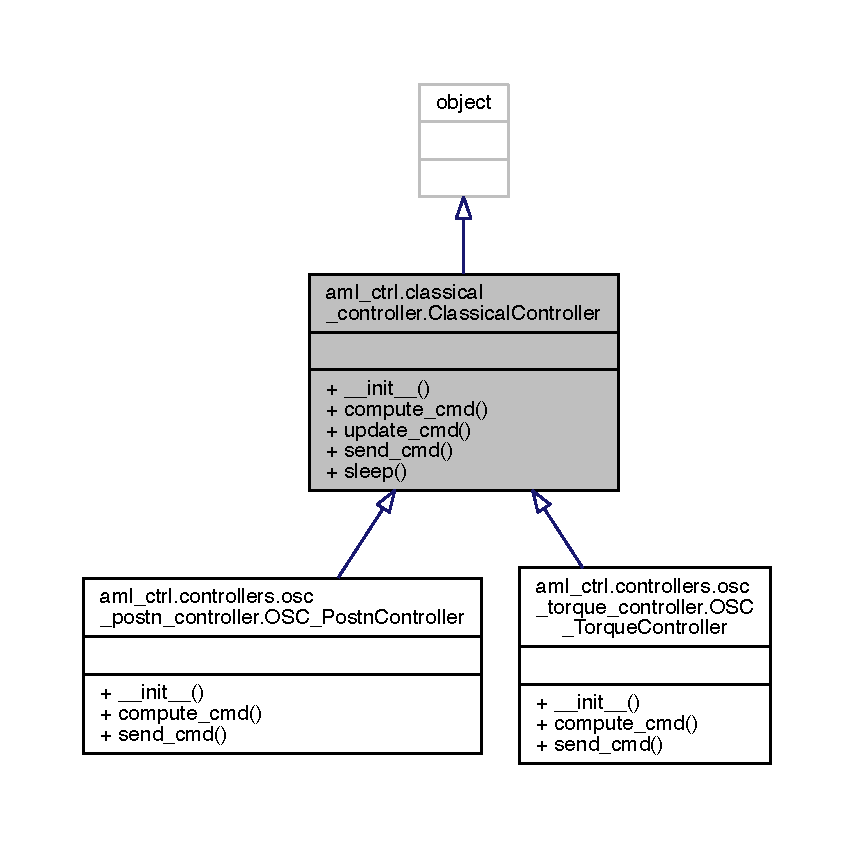
\includegraphics[width=350pt]{classaml__ctrl_1_1classical__controller_1_1_classical_controller__inherit__graph}
\end{center}
\end{figure}


Collaboration diagram for aml\+\_\+ctrl.\+classical\+\_\+controller.\+Classical\+Controller\+:
\nopagebreak
\begin{figure}[H]
\begin{center}
\leavevmode
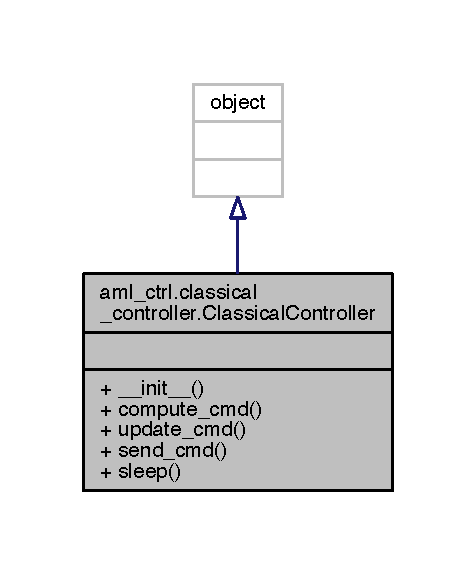
\includegraphics[width=228pt]{classaml__ctrl_1_1classical__controller_1_1_classical_controller__coll__graph}
\end{center}
\end{figure}
\subsection*{Public Member Functions}
\begin{DoxyCompactItemize}
\item 
\hypertarget{classaml__ctrl_1_1classical__controller_1_1_classical_controller_a652f6f673d2d455dc751f1d9f5b2235e}{}\label{classaml__ctrl_1_1classical__controller_1_1_classical_controller_a652f6f673d2d455dc751f1d9f5b2235e} 
def {\bfseries \+\_\+\+\_\+init\+\_\+\+\_\+} (self, robot\+\_\+interface)
\item 
\hypertarget{classaml__ctrl_1_1classical__controller_1_1_classical_controller_a3706654f88e9cea399c7b5912662af68}{}\label{classaml__ctrl_1_1classical__controller_1_1_classical_controller_a3706654f88e9cea399c7b5912662af68} 
def {\bfseries compute\+\_\+cmd} (self, goal\+\_\+pos, goal\+\_\+ori, orientation\+\_\+ctrl)
\item 
\hypertarget{classaml__ctrl_1_1classical__controller_1_1_classical_controller_a25b72cfd5c2bd9d9c9dbc9a2ef19d09f}{}\label{classaml__ctrl_1_1classical__controller_1_1_classical_controller_a25b72cfd5c2bd9d9c9dbc9a2ef19d09f} 
def {\bfseries update\+\_\+cmd} (self)
\item 
\hypertarget{classaml__ctrl_1_1classical__controller_1_1_classical_controller_a0ae03e19f0583e154f65cabcab0b84c8}{}\label{classaml__ctrl_1_1classical__controller_1_1_classical_controller_a0ae03e19f0583e154f65cabcab0b84c8} 
def {\bfseries send\+\_\+cmd} (self)
\item 
\hypertarget{classaml__ctrl_1_1classical__controller_1_1_classical_controller_a355da8c44f2f193aa2fda6f1bbf3bafb}{}\label{classaml__ctrl_1_1classical__controller_1_1_classical_controller_a355da8c44f2f193aa2fda6f1bbf3bafb} 
def {\bfseries sleep} (self)
\end{DoxyCompactItemize}


The documentation for this class was generated from the following file\+:\begin{DoxyCompactItemize}
\item 
aml\+\_\+robot/src/aml\+\_\+ctrl/classical\+\_\+controller.\+py\end{DoxyCompactItemize}

\hypertarget{class_marker_odometry}{}\section{Marker\+Odometry Class Reference}
\label{class_marker_odometry}\index{Marker\+Odometry@{Marker\+Odometry}}


Collaboration diagram for Marker\+Odometry\+:\nopagebreak
\begin{figure}[H]
\begin{center}
\leavevmode
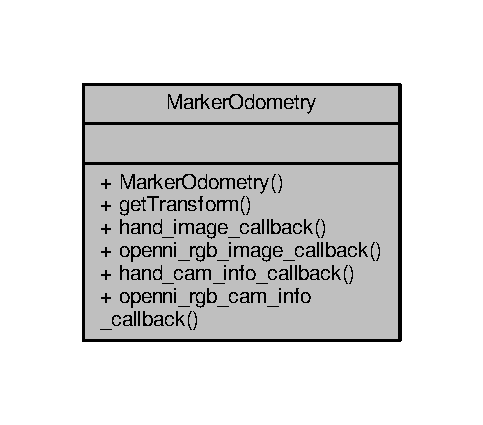
\includegraphics[width=236pt]{class_marker_odometry__coll__graph}
\end{center}
\end{figure}
\subsection*{Public Member Functions}
\begin{DoxyCompactItemize}
\item 
\hypertarget{class_marker_odometry_a991ccdf619ec3c08249f0e8c7b1dfb16}{}\label{class_marker_odometry_a991ccdf619ec3c08249f0e8c7b1dfb16} 
bool {\bfseries get\+Transform} (const std\+::string \&ref\+Frame, const std\+::string \&child\+Frame, tf\+::\+Stamped\+Transform \&transform)
\item 
\hypertarget{class_marker_odometry_a09b1b3528307aa9d2fb98b7e8c923009}{}\label{class_marker_odometry_a09b1b3528307aa9d2fb98b7e8c923009} 
void {\bfseries hand\+\_\+image\+\_\+callback} (const sensor\+\_\+msgs\+::\+Image\+Const\+Ptr \&msg)
\item 
\hypertarget{class_marker_odometry_af6619fc8e9f0183bac7dc40c3a07d097}{}\label{class_marker_odometry_af6619fc8e9f0183bac7dc40c3a07d097} 
void {\bfseries openni\+\_\+rgb\+\_\+image\+\_\+callback} (const sensor\+\_\+msgs\+::\+Image\+Const\+Ptr \&msg)
\item 
\hypertarget{class_marker_odometry_adc0d7677298bed19a3b6a56667c36aeb}{}\label{class_marker_odometry_adc0d7677298bed19a3b6a56667c36aeb} 
void {\bfseries hand\+\_\+cam\+\_\+info\+\_\+callback} (const sensor\+\_\+msgs\+::\+Camera\+Info \&msg)
\item 
\hypertarget{class_marker_odometry_a90f3cc35183a070f578f7f1f57b6c0d8}{}\label{class_marker_odometry_a90f3cc35183a070f578f7f1f57b6c0d8} 
void {\bfseries openni\+\_\+rgb\+\_\+cam\+\_\+info\+\_\+callback} (const sensor\+\_\+msgs\+::\+Camera\+Info \&msg)
\end{DoxyCompactItemize}


The documentation for this class was generated from the following file\+:\begin{DoxyCompactItemize}
\item 
aml\+\_\+calib/src/Marker\+Odometry\+Node.\+cpp\end{DoxyCompactItemize}

\hypertarget{classaml__ctrl_1_1classical__controllers_1_1_min_jerk_controller}{}\section{aml\+\_\+ctrl.\+classical\+\_\+controllers.\+Min\+Jerk\+Controller Class Reference}
\label{classaml__ctrl_1_1classical__controllers_1_1_min_jerk_controller}\index{aml\+\_\+ctrl.\+classical\+\_\+controllers.\+Min\+Jerk\+Controller@{aml\+\_\+ctrl.\+classical\+\_\+controllers.\+Min\+Jerk\+Controller}}


Collaboration diagram for aml\+\_\+ctrl.\+classical\+\_\+controllers.\+Min\+Jerk\+Controller\+:
\nopagebreak
\begin{figure}[H]
\begin{center}
\leavevmode
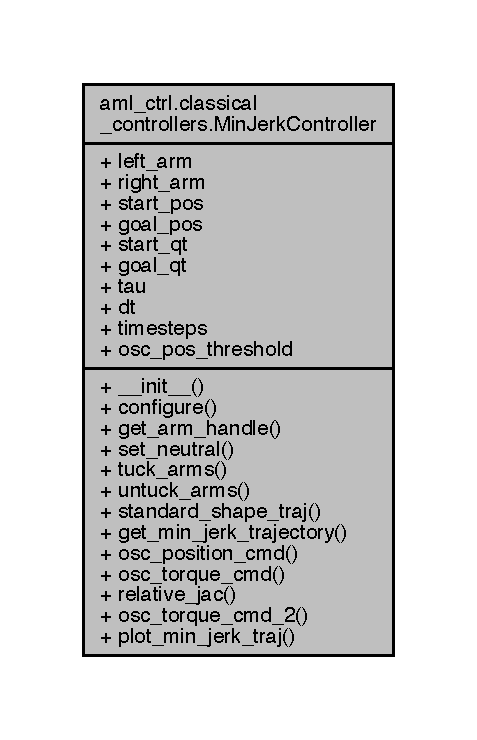
\includegraphics[width=229pt]{classaml__ctrl_1_1classical__controllers_1_1_min_jerk_controller__coll__graph}
\end{center}
\end{figure}
\subsection*{Public Member Functions}
\begin{DoxyCompactItemize}
\item 
\hypertarget{classaml__ctrl_1_1classical__controllers_1_1_min_jerk_controller_a67156f9aad386b58bfc7f471d99cc526}{}\label{classaml__ctrl_1_1classical__controllers_1_1_min_jerk_controller_a67156f9aad386b58bfc7f471d99cc526} 
def {\bfseries \+\_\+\+\_\+init\+\_\+\+\_\+} (self, extern\+\_\+call=False, trial\+\_\+arm=None, aux\+\_\+arm=None, tau=5., dt=0.\+05)
\item 
\hypertarget{classaml__ctrl_1_1classical__controllers_1_1_min_jerk_controller_acd75044b827ff71bec15f996077a17b7}{}\label{classaml__ctrl_1_1classical__controllers_1_1_min_jerk_controller_acd75044b827ff71bec15f996077a17b7} 
def {\bfseries configure} (self, start\+\_\+pos, start\+\_\+ori, goal\+\_\+pos, goal\+\_\+ori)
\item 
\hypertarget{classaml__ctrl_1_1classical__controllers_1_1_min_jerk_controller_aa4549f8c58d03aa508ef7f3dd5b8318e}{}\label{classaml__ctrl_1_1classical__controllers_1_1_min_jerk_controller_aa4549f8c58d03aa508ef7f3dd5b8318e} 
def {\bfseries get\+\_\+arm\+\_\+handle} (self, limb\+\_\+idx=0)
\item 
\hypertarget{classaml__ctrl_1_1classical__controllers_1_1_min_jerk_controller_a37671ba5ea1592a2bf3e169c6d060d9d}{}\label{classaml__ctrl_1_1classical__controllers_1_1_min_jerk_controller_a37671ba5ea1592a2bf3e169c6d060d9d} 
def {\bfseries set\+\_\+neutral} (self)
\item 
\hypertarget{classaml__ctrl_1_1classical__controllers_1_1_min_jerk_controller_a33f260a4253ebdeb0c8d2e6701101bc9}{}\label{classaml__ctrl_1_1classical__controllers_1_1_min_jerk_controller_a33f260a4253ebdeb0c8d2e6701101bc9} 
def {\bfseries tuck\+\_\+arms} (self)
\item 
\hypertarget{classaml__ctrl_1_1classical__controllers_1_1_min_jerk_controller_a72d1867cce1d400fc8ce0f4604da7dfc}{}\label{classaml__ctrl_1_1classical__controllers_1_1_min_jerk_controller_a72d1867cce1d400fc8ce0f4604da7dfc} 
def {\bfseries untuck\+\_\+arms} (self)
\item 
\hypertarget{classaml__ctrl_1_1classical__controllers_1_1_min_jerk_controller_a825535b9b198ad177f27d5d5689ad419}{}\label{classaml__ctrl_1_1classical__controllers_1_1_min_jerk_controller_a825535b9b198ad177f27d5d5689ad419} 
def {\bfseries standard\+\_\+shape\+\_\+traj} (self, curr\+\_\+pos, no\+\_\+set\+\_\+points=16, shape=\textquotesingle{}circle\textquotesingle{})
\item 
\hypertarget{classaml__ctrl_1_1classical__controllers_1_1_min_jerk_controller_affaeff25c410f9d0617b551392c4fcdf}{}\label{classaml__ctrl_1_1classical__controllers_1_1_min_jerk_controller_affaeff25c410f9d0617b551392c4fcdf} 
def {\bfseries get\+\_\+min\+\_\+jerk\+\_\+trajectory} (self)
\item 
\hypertarget{classaml__ctrl_1_1classical__controllers_1_1_min_jerk_controller_aa4cdd987c45c52d39f38ec3ff83f8f1d}{}\label{classaml__ctrl_1_1classical__controllers_1_1_min_jerk_controller_aa4cdd987c45c52d39f38ec3ff83f8f1d} 
def {\bfseries osc\+\_\+position\+\_\+cmd} (self, goal\+\_\+pos, goal\+\_\+ori=None, limb\+\_\+idx=0, orientation\+\_\+ctrl=False)
\item 
\hypertarget{classaml__ctrl_1_1classical__controllers_1_1_min_jerk_controller_a54182a9ca601563ef471063650978820}{}\label{classaml__ctrl_1_1classical__controllers_1_1_min_jerk_controller_a54182a9ca601563ef471063650978820} 
def {\bfseries osc\+\_\+torque\+\_\+cmd} (self, goal\+\_\+pos, goal\+\_\+ori=None, limb\+\_\+idx=0, orientation\+\_\+ctrl=False)
\item 
\hypertarget{classaml__ctrl_1_1classical__controllers_1_1_min_jerk_controller_a9b88c1b2a047a254b7e59c4cc0627995}{}\label{classaml__ctrl_1_1classical__controllers_1_1_min_jerk_controller_a9b88c1b2a047a254b7e59c4cc0627995} 
def {\bfseries relative\+\_\+jac} (self, rel\+\_\+pos)
\item 
\hypertarget{classaml__ctrl_1_1classical__controllers_1_1_min_jerk_controller_a05fe88df81c713f6d4a4eb683c463f57}{}\label{classaml__ctrl_1_1classical__controllers_1_1_min_jerk_controller_a05fe88df81c713f6d4a4eb683c463f57} 
def {\bfseries osc\+\_\+torque\+\_\+cmd\+\_\+2} (self, arm\+\_\+data, goal\+\_\+pos, goal\+\_\+ori=None, orientation\+\_\+ctrl=False)
\item 
\hypertarget{classaml__ctrl_1_1classical__controllers_1_1_min_jerk_controller_a8f6ff35c217c121c2de2e805c173845b}{}\label{classaml__ctrl_1_1classical__controllers_1_1_min_jerk_controller_a8f6ff35c217c121c2de2e805c173845b} 
def {\bfseries plot\+\_\+min\+\_\+jerk\+\_\+traj} (self)
\end{DoxyCompactItemize}
\subsection*{Public Attributes}
\begin{DoxyCompactItemize}
\item 
\hypertarget{classaml__ctrl_1_1classical__controllers_1_1_min_jerk_controller_aabe9d1a061a6f6cb9b26979e2a93c7c6}{}\label{classaml__ctrl_1_1classical__controllers_1_1_min_jerk_controller_aabe9d1a061a6f6cb9b26979e2a93c7c6} 
{\bfseries left\+\_\+arm}
\item 
\hypertarget{classaml__ctrl_1_1classical__controllers_1_1_min_jerk_controller_a2f49b270f60da2410036f62b293643a1}{}\label{classaml__ctrl_1_1classical__controllers_1_1_min_jerk_controller_a2f49b270f60da2410036f62b293643a1} 
{\bfseries right\+\_\+arm}
\item 
\hypertarget{classaml__ctrl_1_1classical__controllers_1_1_min_jerk_controller_a51a6ea302e41b4ced13f44a8ed1873f9}{}\label{classaml__ctrl_1_1classical__controllers_1_1_min_jerk_controller_a51a6ea302e41b4ced13f44a8ed1873f9} 
{\bfseries start\+\_\+pos}
\item 
\hypertarget{classaml__ctrl_1_1classical__controllers_1_1_min_jerk_controller_a457eed8bb3e71b2ce6da0a3f470f37b4}{}\label{classaml__ctrl_1_1classical__controllers_1_1_min_jerk_controller_a457eed8bb3e71b2ce6da0a3f470f37b4} 
{\bfseries goal\+\_\+pos}
\item 
\hypertarget{classaml__ctrl_1_1classical__controllers_1_1_min_jerk_controller_a7c27621e163f2c438c1b76cfb9477e82}{}\label{classaml__ctrl_1_1classical__controllers_1_1_min_jerk_controller_a7c27621e163f2c438c1b76cfb9477e82} 
{\bfseries start\+\_\+qt}
\item 
\hypertarget{classaml__ctrl_1_1classical__controllers_1_1_min_jerk_controller_a1b557c17e8356729fb179ab67ec0d1d1}{}\label{classaml__ctrl_1_1classical__controllers_1_1_min_jerk_controller_a1b557c17e8356729fb179ab67ec0d1d1} 
{\bfseries goal\+\_\+qt}
\item 
\hypertarget{classaml__ctrl_1_1classical__controllers_1_1_min_jerk_controller_a23a689c23418cac10b3ad373eec3dcd0}{}\label{classaml__ctrl_1_1classical__controllers_1_1_min_jerk_controller_a23a689c23418cac10b3ad373eec3dcd0} 
{\bfseries tau}
\item 
\hypertarget{classaml__ctrl_1_1classical__controllers_1_1_min_jerk_controller_aceb3147e0da967bfc101ea5a1e6489a5}{}\label{classaml__ctrl_1_1classical__controllers_1_1_min_jerk_controller_aceb3147e0da967bfc101ea5a1e6489a5} 
{\bfseries dt}
\item 
\hypertarget{classaml__ctrl_1_1classical__controllers_1_1_min_jerk_controller_aedd1be03de0d0d6707a5b94716123b3b}{}\label{classaml__ctrl_1_1classical__controllers_1_1_min_jerk_controller_aedd1be03de0d0d6707a5b94716123b3b} 
{\bfseries timesteps}
\item 
\hypertarget{classaml__ctrl_1_1classical__controllers_1_1_min_jerk_controller_a409c6319b72e2f79bb962f9d1a69cf12}{}\label{classaml__ctrl_1_1classical__controllers_1_1_min_jerk_controller_a409c6319b72e2f79bb962f9d1a69cf12} 
{\bfseries osc\+\_\+pos\+\_\+threshold}
\end{DoxyCompactItemize}


The documentation for this class was generated from the following file\+:\begin{DoxyCompactItemize}
\item 
aml\+\_\+robot/src/aml\+\_\+ctrl/classical\+\_\+controllers.\+py\end{DoxyCompactItemize}

\hypertarget{classaml__ctrl_1_1utilities_1_1min__jerk__interp_1_1_min_jerk_interp}{}\section{aml\+\_\+ctrl.\+utilities.\+min\+\_\+jerk\+\_\+interp.\+Min\+Jerk\+Interp Class Reference}
\label{classaml__ctrl_1_1utilities_1_1min__jerk__interp_1_1_min_jerk_interp}\index{aml\+\_\+ctrl.\+utilities.\+min\+\_\+jerk\+\_\+interp.\+Min\+Jerk\+Interp@{aml\+\_\+ctrl.\+utilities.\+min\+\_\+jerk\+\_\+interp.\+Min\+Jerk\+Interp}}


Collaboration diagram for aml\+\_\+ctrl.\+utilities.\+min\+\_\+jerk\+\_\+interp.\+Min\+Jerk\+Interp\+:
\nopagebreak
\begin{figure}[H]
\begin{center}
\leavevmode
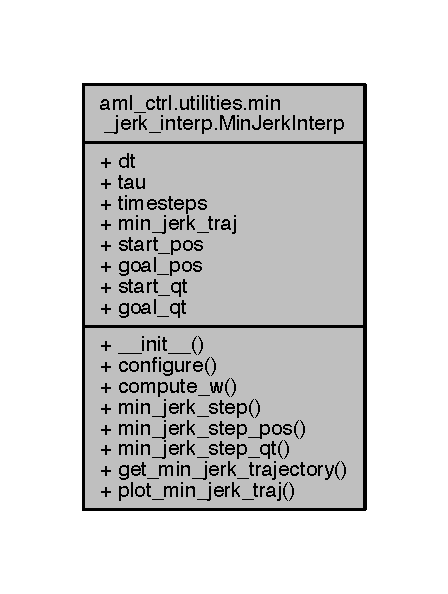
\includegraphics[width=215pt]{classaml__ctrl_1_1utilities_1_1min__jerk__interp_1_1_min_jerk_interp__coll__graph}
\end{center}
\end{figure}
\subsection*{Public Member Functions}
\begin{DoxyCompactItemize}
\item 
\hypertarget{classaml__ctrl_1_1utilities_1_1min__jerk__interp_1_1_min_jerk_interp_aadf63d0220915bfd457f26caaeedb52c}{}\label{classaml__ctrl_1_1utilities_1_1min__jerk__interp_1_1_min_jerk_interp_aadf63d0220915bfd457f26caaeedb52c} 
def {\bfseries \+\_\+\+\_\+init\+\_\+\+\_\+} (self, dt=0.\+05, tau=5.)
\item 
\hypertarget{classaml__ctrl_1_1utilities_1_1min__jerk__interp_1_1_min_jerk_interp_ad0948202cbfaeb4c69099e8ba32a5b09}{}\label{classaml__ctrl_1_1utilities_1_1min__jerk__interp_1_1_min_jerk_interp_ad0948202cbfaeb4c69099e8ba32a5b09} 
def {\bfseries configure} (self, start\+\_\+pos, start\+\_\+qt, goal\+\_\+pos, goal\+\_\+qt)
\item 
\hypertarget{classaml__ctrl_1_1utilities_1_1min__jerk__interp_1_1_min_jerk_interp_a84ec24d901c9582b4151de75b9b02b83}{}\label{classaml__ctrl_1_1utilities_1_1min__jerk__interp_1_1_min_jerk_interp_a84ec24d901c9582b4151de75b9b02b83} 
def {\bfseries compute\+\_\+w} (self, q, qdot)
\item 
\hypertarget{classaml__ctrl_1_1utilities_1_1min__jerk__interp_1_1_min_jerk_interp_a5620dafe71bfe0d1908dd810d01e846d}{}\label{classaml__ctrl_1_1utilities_1_1min__jerk__interp_1_1_min_jerk_interp_a5620dafe71bfe0d1908dd810d01e846d} 
def {\bfseries min\+\_\+jerk\+\_\+step} (self, x, xd, xdd, goal, tau)
\item 
\hypertarget{classaml__ctrl_1_1utilities_1_1min__jerk__interp_1_1_min_jerk_interp_a0c3279ef71e9e83355604f8c754ae5b7}{}\label{classaml__ctrl_1_1utilities_1_1min__jerk__interp_1_1_min_jerk_interp_a0c3279ef71e9e83355604f8c754ae5b7} 
def {\bfseries min\+\_\+jerk\+\_\+step\+\_\+pos} (self)
\item 
\hypertarget{classaml__ctrl_1_1utilities_1_1min__jerk__interp_1_1_min_jerk_interp_a5888e83ccea393d6775a684f44104489}{}\label{classaml__ctrl_1_1utilities_1_1min__jerk__interp_1_1_min_jerk_interp_a5888e83ccea393d6775a684f44104489} 
def {\bfseries min\+\_\+jerk\+\_\+step\+\_\+qt} (self)
\item 
\hypertarget{classaml__ctrl_1_1utilities_1_1min__jerk__interp_1_1_min_jerk_interp_a06e9332a4367aa9db11f4d3557a203c9}{}\label{classaml__ctrl_1_1utilities_1_1min__jerk__interp_1_1_min_jerk_interp_a06e9332a4367aa9db11f4d3557a203c9} 
def {\bfseries get\+\_\+min\+\_\+jerk\+\_\+trajectory} (self)
\item 
\hypertarget{classaml__ctrl_1_1utilities_1_1min__jerk__interp_1_1_min_jerk_interp_ab4470625eaf22769bdc5f20e914ad5dd}{}\label{classaml__ctrl_1_1utilities_1_1min__jerk__interp_1_1_min_jerk_interp_ab4470625eaf22769bdc5f20e914ad5dd} 
def {\bfseries plot\+\_\+min\+\_\+jerk\+\_\+traj} (self)
\end{DoxyCompactItemize}
\subsection*{Public Attributes}
\begin{DoxyCompactItemize}
\item 
\hypertarget{classaml__ctrl_1_1utilities_1_1min__jerk__interp_1_1_min_jerk_interp_a3cf50dd857ae275c6a9309c560a334f0}{}\label{classaml__ctrl_1_1utilities_1_1min__jerk__interp_1_1_min_jerk_interp_a3cf50dd857ae275c6a9309c560a334f0} 
{\bfseries dt}
\item 
\hypertarget{classaml__ctrl_1_1utilities_1_1min__jerk__interp_1_1_min_jerk_interp_abfbc4183bd40597d1f8ef549c8a954cd}{}\label{classaml__ctrl_1_1utilities_1_1min__jerk__interp_1_1_min_jerk_interp_abfbc4183bd40597d1f8ef549c8a954cd} 
{\bfseries tau}
\item 
\hypertarget{classaml__ctrl_1_1utilities_1_1min__jerk__interp_1_1_min_jerk_interp_a53f374cd9afb16fb0293c4f65987795d}{}\label{classaml__ctrl_1_1utilities_1_1min__jerk__interp_1_1_min_jerk_interp_a53f374cd9afb16fb0293c4f65987795d} 
{\bfseries timesteps}
\item 
\hypertarget{classaml__ctrl_1_1utilities_1_1min__jerk__interp_1_1_min_jerk_interp_a655ecaf3042fd23a9dea45fcac07c520}{}\label{classaml__ctrl_1_1utilities_1_1min__jerk__interp_1_1_min_jerk_interp_a655ecaf3042fd23a9dea45fcac07c520} 
{\bfseries min\+\_\+jerk\+\_\+traj}
\item 
\hypertarget{classaml__ctrl_1_1utilities_1_1min__jerk__interp_1_1_min_jerk_interp_a2154616a9adab36c591fc90b62ac66cc}{}\label{classaml__ctrl_1_1utilities_1_1min__jerk__interp_1_1_min_jerk_interp_a2154616a9adab36c591fc90b62ac66cc} 
{\bfseries start\+\_\+pos}
\item 
\hypertarget{classaml__ctrl_1_1utilities_1_1min__jerk__interp_1_1_min_jerk_interp_af33d73bed61d6eebe0ddbb1ca953a881}{}\label{classaml__ctrl_1_1utilities_1_1min__jerk__interp_1_1_min_jerk_interp_af33d73bed61d6eebe0ddbb1ca953a881} 
{\bfseries goal\+\_\+pos}
\item 
\hypertarget{classaml__ctrl_1_1utilities_1_1min__jerk__interp_1_1_min_jerk_interp_a1d7c1d1cc8b9b64922061d060d331d8a}{}\label{classaml__ctrl_1_1utilities_1_1min__jerk__interp_1_1_min_jerk_interp_a1d7c1d1cc8b9b64922061d060d331d8a} 
{\bfseries start\+\_\+qt}
\item 
\hypertarget{classaml__ctrl_1_1utilities_1_1min__jerk__interp_1_1_min_jerk_interp_a6aa537ca52a3e35e06ef582303e4501f}{}\label{classaml__ctrl_1_1utilities_1_1min__jerk__interp_1_1_min_jerk_interp_a6aa537ca52a3e35e06ef582303e4501f} 
{\bfseries goal\+\_\+qt}
\end{DoxyCompactItemize}


The documentation for this class was generated from the following file\+:\begin{DoxyCompactItemize}
\item 
aml\+\_\+robot/src/aml\+\_\+ctrl/utilities/min\+\_\+jerk\+\_\+interp.\+py\end{DoxyCompactItemize}

\hypertarget{classaml__ctrl_1_1controllers_1_1osc__postn__controller_1_1_o_s_c___postn_controller}{}\section{aml\+\_\+ctrl.\+controllers.\+osc\+\_\+postn\+\_\+controller.\+O\+S\+C\+\_\+\+Postn\+Controller Class Reference}
\label{classaml__ctrl_1_1controllers_1_1osc__postn__controller_1_1_o_s_c___postn_controller}\index{aml\+\_\+ctrl.\+controllers.\+osc\+\_\+postn\+\_\+controller.\+O\+S\+C\+\_\+\+Postn\+Controller@{aml\+\_\+ctrl.\+controllers.\+osc\+\_\+postn\+\_\+controller.\+O\+S\+C\+\_\+\+Postn\+Controller}}


Inheritance diagram for aml\+\_\+ctrl.\+controllers.\+osc\+\_\+postn\+\_\+controller.\+O\+S\+C\+\_\+\+Postn\+Controller\+:
\nopagebreak
\begin{figure}[H]
\begin{center}
\leavevmode
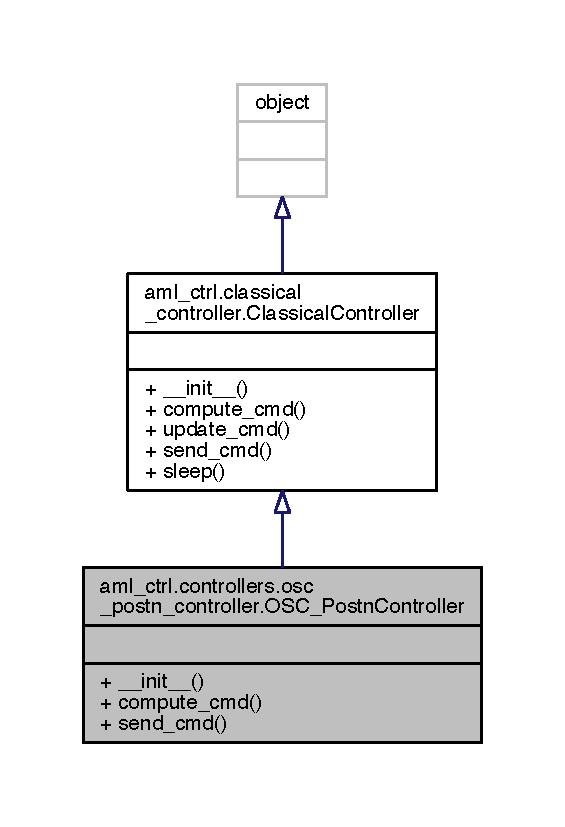
\includegraphics[width=271pt]{classaml__ctrl_1_1controllers_1_1osc__postn__controller_1_1_o_s_c___postn_controller__inherit__graph}
\end{center}
\end{figure}


Collaboration diagram for aml\+\_\+ctrl.\+controllers.\+osc\+\_\+postn\+\_\+controller.\+O\+S\+C\+\_\+\+Postn\+Controller\+:
\nopagebreak
\begin{figure}[H]
\begin{center}
\leavevmode
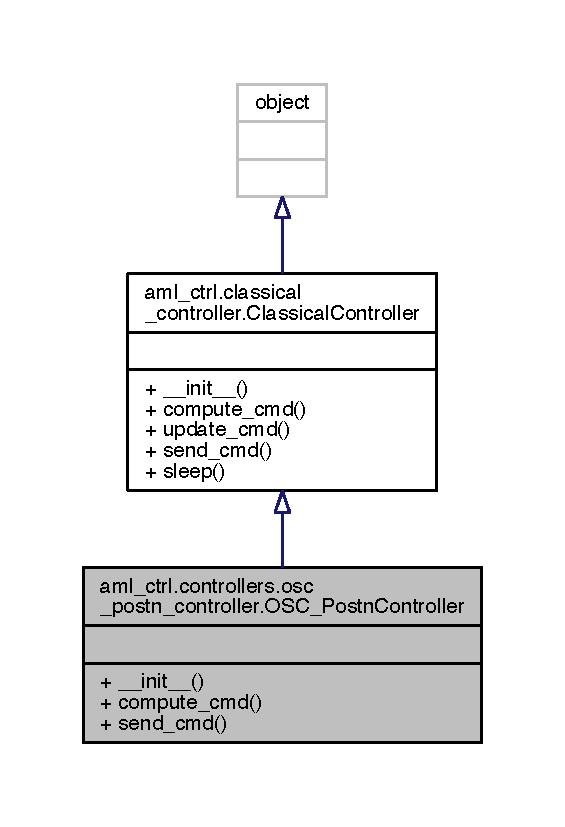
\includegraphics[width=271pt]{classaml__ctrl_1_1controllers_1_1osc__postn__controller_1_1_o_s_c___postn_controller__coll__graph}
\end{center}
\end{figure}
\subsection*{Public Member Functions}
\begin{DoxyCompactItemize}
\item 
\hypertarget{classaml__ctrl_1_1controllers_1_1osc__postn__controller_1_1_o_s_c___postn_controller_a675e78b93e74ca6703cc5dbaa7bb551b}{}\label{classaml__ctrl_1_1controllers_1_1osc__postn__controller_1_1_o_s_c___postn_controller_a675e78b93e74ca6703cc5dbaa7bb551b} 
def {\bfseries \+\_\+\+\_\+init\+\_\+\+\_\+} (self, robot\+\_\+interface)
\item 
\hypertarget{classaml__ctrl_1_1controllers_1_1osc__postn__controller_1_1_o_s_c___postn_controller_a77b1a1bd3104b8b6da36ca477ce2fef0}{}\label{classaml__ctrl_1_1controllers_1_1osc__postn__controller_1_1_o_s_c___postn_controller_a77b1a1bd3104b8b6da36ca477ce2fef0} 
def {\bfseries compute\+\_\+cmd} (self, goal\+\_\+pos, goal\+\_\+ori, orientation\+\_\+ctrl=False)
\item 
\hypertarget{classaml__ctrl_1_1controllers_1_1osc__postn__controller_1_1_o_s_c___postn_controller_a09312be058926405ac24dbf886889f58}{}\label{classaml__ctrl_1_1controllers_1_1osc__postn__controller_1_1_o_s_c___postn_controller_a09312be058926405ac24dbf886889f58} 
def {\bfseries send\+\_\+cmd} (self)
\end{DoxyCompactItemize}


The documentation for this class was generated from the following file\+:\begin{DoxyCompactItemize}
\item 
aml\+\_\+robot/src/aml\+\_\+ctrl/controllers/osc\+\_\+postn\+\_\+controller.\+py\end{DoxyCompactItemize}

\hypertarget{classaml__ctrl_1_1controllers_1_1osc__torque__controller_1_1_o_s_c___torque_controller}{}\section{aml\+\_\+ctrl.\+controllers.\+osc\+\_\+torque\+\_\+controller.\+O\+S\+C\+\_\+\+Torque\+Controller Class Reference}
\label{classaml__ctrl_1_1controllers_1_1osc__torque__controller_1_1_o_s_c___torque_controller}\index{aml\+\_\+ctrl.\+controllers.\+osc\+\_\+torque\+\_\+controller.\+O\+S\+C\+\_\+\+Torque\+Controller@{aml\+\_\+ctrl.\+controllers.\+osc\+\_\+torque\+\_\+controller.\+O\+S\+C\+\_\+\+Torque\+Controller}}


Inheritance diagram for aml\+\_\+ctrl.\+controllers.\+osc\+\_\+torque\+\_\+controller.\+O\+S\+C\+\_\+\+Torque\+Controller\+:
\nopagebreak
\begin{figure}[H]
\begin{center}
\leavevmode
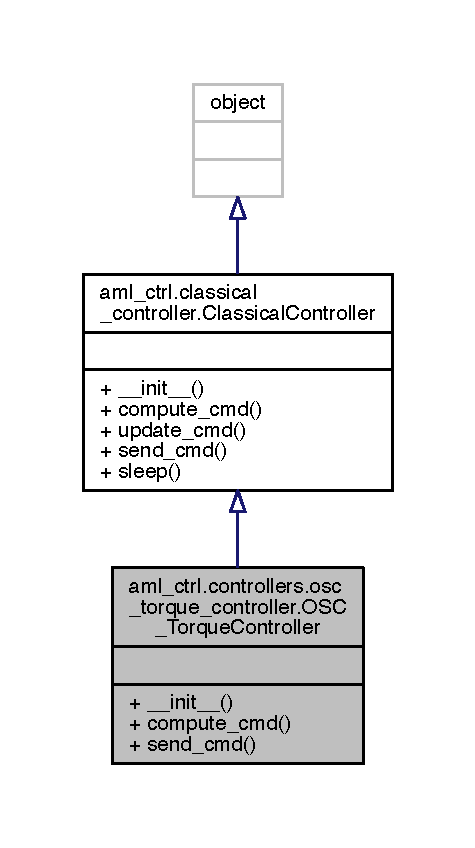
\includegraphics[width=228pt]{classaml__ctrl_1_1controllers_1_1osc__torque__controller_1_1_o_s_c___torque_controller__inherit__graph}
\end{center}
\end{figure}


Collaboration diagram for aml\+\_\+ctrl.\+controllers.\+osc\+\_\+torque\+\_\+controller.\+O\+S\+C\+\_\+\+Torque\+Controller\+:
\nopagebreak
\begin{figure}[H]
\begin{center}
\leavevmode
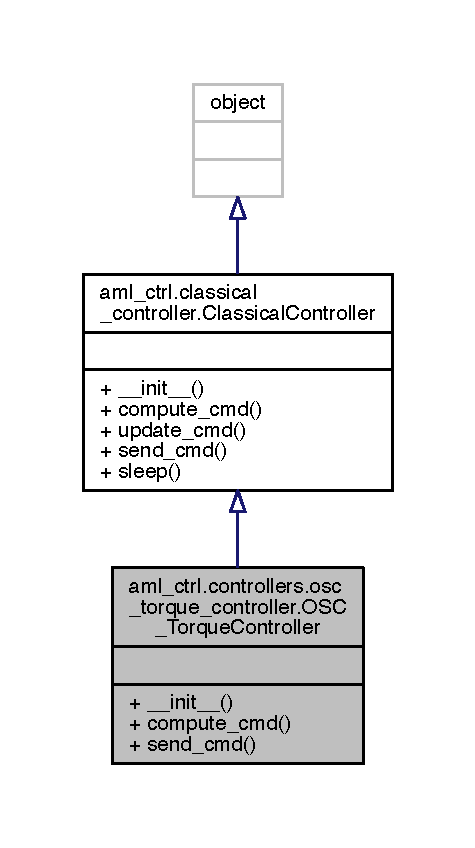
\includegraphics[width=228pt]{classaml__ctrl_1_1controllers_1_1osc__torque__controller_1_1_o_s_c___torque_controller__coll__graph}
\end{center}
\end{figure}
\subsection*{Public Member Functions}
\begin{DoxyCompactItemize}
\item 
\hypertarget{classaml__ctrl_1_1controllers_1_1osc__torque__controller_1_1_o_s_c___torque_controller_af8968b14f9ff120ae0d3ec3683871efa}{}\label{classaml__ctrl_1_1controllers_1_1osc__torque__controller_1_1_o_s_c___torque_controller_af8968b14f9ff120ae0d3ec3683871efa} 
def {\bfseries \+\_\+\+\_\+init\+\_\+\+\_\+} (self, robot\+\_\+interface)
\item 
\hypertarget{classaml__ctrl_1_1controllers_1_1osc__torque__controller_1_1_o_s_c___torque_controller_aab342800c6930d53833c67ea1b05798f}{}\label{classaml__ctrl_1_1controllers_1_1osc__torque__controller_1_1_o_s_c___torque_controller_aab342800c6930d53833c67ea1b05798f} 
def {\bfseries compute\+\_\+cmd} (self, goal\+\_\+pos, goal\+\_\+ori, orientation\+\_\+ctrl=False)
\item 
\hypertarget{classaml__ctrl_1_1controllers_1_1osc__torque__controller_1_1_o_s_c___torque_controller_a2c4085b111ce0db1b63f3883caac977a}{}\label{classaml__ctrl_1_1controllers_1_1osc__torque__controller_1_1_o_s_c___torque_controller_a2c4085b111ce0db1b63f3883caac977a} 
def {\bfseries send\+\_\+cmd} (self)
\end{DoxyCompactItemize}


The documentation for this class was generated from the following file\+:\begin{DoxyCompactItemize}
\item 
aml\+\_\+robot/src/aml\+\_\+ctrl/controllers/osc\+\_\+torque\+\_\+controller.\+py\end{DoxyCompactItemize}

\hypertarget{classtests_1_1_some_obj}{}\section{tests.\+Some\+Obj Class Reference}
\label{classtests_1_1_some_obj}\index{tests.\+Some\+Obj@{tests.\+Some\+Obj}}


Collaboration diagram for tests.\+Some\+Obj\+:\nopagebreak
\begin{figure}[H]
\begin{center}
\leavevmode
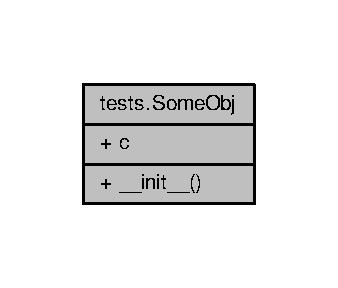
\includegraphics[width=162pt]{classtests_1_1_some_obj__coll__graph}
\end{center}
\end{figure}
\subsection*{Public Member Functions}
\begin{DoxyCompactItemize}
\item 
\hypertarget{classtests_1_1_some_obj_a6bbab9d4ef4c83ef011a468be214639d}{}\label{classtests_1_1_some_obj_a6bbab9d4ef4c83ef011a468be214639d} 
def {\bfseries \+\_\+\+\_\+init\+\_\+\+\_\+} (self)
\end{DoxyCompactItemize}
\subsection*{Public Attributes}
\begin{DoxyCompactItemize}
\item 
\hypertarget{classtests_1_1_some_obj_ad442c35720f3dd0172c277d3bb4e9316}{}\label{classtests_1_1_some_obj_ad442c35720f3dd0172c277d3bb4e9316} 
{\bfseries c}
\end{DoxyCompactItemize}


The documentation for this class was generated from the following file\+:\begin{DoxyCompactItemize}
\item 
aml\+\_\+robot/src/tests.\+py\end{DoxyCompactItemize}

%--- End generated contents ---

% Index
\backmatter
\newpage
\phantomsection
\clearemptydoublepage
\addcontentsline{toc}{chapter}{Index}
\printindex

\end{document}
